\documentclass[12pt]{report}

\usepackage[top=2cm, bottom=2cm, left=3.5cm, right=2cm, a4paper]{geometry}
\usepackage{titletoc}
\usepackage{tikz}
\usepackage{epigraph}
\usepackage{xpatch}
\usepackage{lmodern}
\usepackage[utf8]{vietnam}
\usepackage{ragged2e}
\usepackage{fancyhdr}
\usepackage[hidelinks]{hyperref}
\usepackage{float}
\usepackage{array}
\usepackage{amssymb}
\usepackage{amsmath}
\newcolumntype{C}{>{\centering\arraybackslash}m{3cm}}

%source codes
\definecolor{bluekeywords}{rgb}{0.13,0.13,1}
\definecolor{greencomments}{rgb}{0,0.5,0}
\definecolor{redstrings}{rgb}{0.9,0,0}

\usepackage{listingsutf8}
\lstset{language=[Sharp]C,
showspaces=false,
showtabs=false,
breaklines=true,
showstringspaces=false,
breakatwhitespace=true,
escapeinside={(*@}{@*)},
commentstyle=\color{greencomments},
keywordstyle=\color{bluekeywords}\bfseries,
stringstyle=\color{redstrings},
basicstyle=\ttfamily
    backgroundcolor=\color{background},
}
\usepackage{xcolor}

\colorlet{punct}{red!60!black}
\definecolor{background}{HTML}{EEEEEE}
\definecolor{delim}{RGB}{20,105,176}
\colorlet{numb}{magenta!60!black}
\lstdefinelanguage{json}{
    basicstyle=\normalfont\ttfamily,
    numbers=left,
    numberstyle=\scriptsize,
    stepnumber=1,
    numbersep=8pt,
    showstringspaces=false,
    breaklines=true,
    frame=lines,
    backgroundcolor=\color{background},
    literate=
     *{0}{{{\color{numb}0}}}{1}
      {1}{{{\color{numb}1}}}{1}
      {2}{{{\color{numb}2}}}{1}
      {3}{{{\color{numb}3}}}{1}
      {4}{{{\color{numb}4}}}{1}
      {5}{{{\color{numb}5}}}{1}
      {6}{{{\color{numb}6}}}{1}
      {7}{{{\color{numb}7}}}{1}
      {8}{{{\color{numb}8}}}{1}
      {9}{{{\color{numb}9}}}{1}
      {:}{{{\color{punct}{:}}}}{1}
      {,}{{{\color{punct}{,}}}}{1}
      {\{}{{{\color{delim}{\{}}}}{1}
      {\}}{{{\color{delim}{\}}}}}{1}
      {[}{{{\color{delim}{[}}}}{1}
      {]}{{{\color{delim}{]}}}}{1},
}

\renewcommand{\lstlistingname}{Mã nguồn}
\renewcommand{\lstlistlistingname}{Danh sách mã nguồn}

% Part ToC
\usepackage{titlesec,titletoc}  

\titleclass{\part}{top}
\titleformat{\part}
[display]
{\centering\normalfont\Huge\bfseries}
{\titlerule[2pt]\vspace{15pt}\MakeUppercase{\partname} \thepart}
{0pt}
{\vspace{1pc}\LARGE}[{\vspace{1pc}\titlerule[1pt]}]

\setcounter{secnumdepth}{5}


%Vietnamese
\usepackage[utf8]{inputenc}

%Line spacing
\renewcommand{\baselinestretch}{1.2}
\usepackage{tikz}
\usetikzlibrary{calc}
\newcommand\HRule{\rule{\textwidth}{1pt}}

%Page style
\pagestyle{fancy}
\fancyhf{}
\rhead{}
\lhead{}
\lfoot{\textit{Sinh viên thực hiện: Trần Hoài Nam, 20122123, CNTT2 04 K57}}
\rfoot{\thepage}
\renewcommand{\footrulewidth}{1pt}

% Redefine the plain page style
% \fancypagestyle{plain}{%
%   \fancyhf{}%
%   \lfoot{\textit{Sinh viên thực hiện: Trần Hoài Nam, 20122123, CNTT2 04 K57}}
%   \rfoot{\thepage}
%   \renewcommand{\headrulewidth}{0pt}% Line at the header invisible
%   \renewcommand{\footrulewidth}{1pt}% Line at the footer visible
% }

%ToC page style
\usepackage{tocloft}

\renewcommand\cftsecleader{\cftdotfill{\cftdotsep}}
\renewcommand\cftchapleader{\cftdotfill{\cftdotsep}}
\renewcommand\cftpartleader{\cftdotfill{\cftnodots}}

% Quote box
\usepackage{framed}
\usepackage[strict]{changepage}    

%Defining colour with different models.
\definecolor{lightgray}{gray}{0.95}
\definecolor{mygray}{gray}{0.8} 

\newenvironment{formal}{%
  \def\FrameCommand{%
    \hspace{1pt}%
    {\color{mygray}\vrule width 6pt}%
    {\color{lightgray}\vrule width 4pt}%
    \colorbox{lightgray}%
  }%
  \MakeFramed{\advance\hsize-\width\FrameRestore}%
  \noindent\hspace{-4.55pt}% disable indenting first paragraph
  \begin{adjustwidth}{}{7pt}%
  \vspace{2pt}\vspace{2pt}%
}
{%
  \vspace{2pt}\end{adjustwidth}\endMakeFramed%
}

%Replaceable project name
\newcommand{\project}{VVC}
\newcommand{\thesistitle}{Xây dựng chatbot điều khiển điện thoại bằng Tiếng Việt}

\begin{document}

\begin{titlepage}

	\begin{tikzpicture}[remember picture, overlay]
	  \draw[line width = 1pt] ($(current page.north west) + (3.5cm,-2cm)$) rectangle ($(current page.south east) + (-2cm,2cm)$);
	\end{tikzpicture}

	\begin{center}
		\vspace{0.3cm}
		\begin{large}
		TRƯỜNG ĐẠI HỌC BÁCH KHOA HÀ NỘI	\\
		VIỆN CÔNG NGHỆ THÔNG TIN VÀ TRUYỀN THÔNG	\\
		\_\_\_\_\_\_\_\_*\_\_\_\_\_\_\_\_ \\[4.5cm]
		\end{large}
			
		{\huge ĐỒ ÁN }\\	
		{\Huge \textbf{TỐT NGHIỆP ĐẠI HỌC}}\\[0.3cm]
		{\Large NGÀNH CÔNG NGHỆ THÔNG TIN}  \\[4cm]
	
		{\Large \textbf{ĐỀ TÀI}}\\[0.3cm]		
		{\large XÂY DỰNG CHATBOT ĐIỀU KHIỂN ĐIỆN THOẠI\\[0.1cm]BẰNG TIẾNG VIỆT} \\[2.5cm]
	\end{center}
	
	\begin{justify}

		\hspace{6cm} Sinh viên thực hiện \hspace{0.15cm}: \textbf{Trần Hoài Nam} \hspace{0.3cm}

		\noindent \hspace{6cm} Lớp \hspace{3.0cm}: CNTT-TT2 04, K57 \hspace{0.3cm}

		\noindent \hspace{6cm} Giáo viên hướng dẫn\hspace{0.14cm} : ThS. \textbf{Trịnh Thành Trung} \hspace{0.3cm} \\[2.5cm]
		
	\end{justify}

	\begin{center}
		Hà Nội, 5/2017
	\end{center}
	
\end{titlepage}

\pagenumbering{roman}
\setcounter{page}{1}

% Phiếu giao nhiệm vụ đồ án tốt nghiệp
\begin{center}
{\large \textbf{PHIẾU GIAO NHIỆM VỤ ĐỒ ÁN TỐT NGHIỆP}}
\end{center}

\noindent 1. Thông tin về sinh viên\\[0.2cm]
\noindent \begin{tabular}{p{0.5\textwidth} p{0.5\textwidth}}
Họ và tên sinh viên: Trần Hoài Nam &   \\ 
Điện thoại liên lạc: 0918218111 & Email: \url{namth27494@gmail.com} \\ 
Lớp: CNTT-TT2 04 K57 & Hệ đào tạo: Đại học \\ 
\end{tabular}\\[0.3cm]
\noindent Đồ án tốt nghiệp được thực hiện tại: Viện công nghệ thông tin \& truyền thông - Trường Đại học Bách Khoa Hà Nội.

\noindent Thời gian làm ĐATN: Từ 01/2017 đến 05/2017.\\[0.4cm]
\noindent 2. Mục đích nội dung của ĐATN\\
\noindent \thesistitle{}.\\[0.4cm]
\noindent 3. Các nhiệm vụ cụ thể của ĐATN
\begin{itemize}
	\item Xây dựng chatbot hiểu được yêu cầu từ người dùng bằng Tiếng Việt.
	\item Hỗ trợ giao tiếp bằng giọng nói.
	\item Cải thiện khả năng phân tích giọng nói thành văn bản.
\end{itemize}

\noindent 4. Lời cam đoan của sinh viên:\\
Tôi - \textit{Trần Hoài Nam} - cam kết ĐATN là công trình nghiên cứu của bản thân tôi dươi sự hướng dẫn của \textit{ThS. Trịnh Thành Trung}.

\noindent Các kết quả nêu trong ĐATN là trung thực, không phải là sao chép hoàn văn của bất kỳ công trình nào khác.\\[0.5cm]
  
\begin{minipage}{0.3\textwidth}
\hspace{1cm}
\end{minipage}
~
\begin{minipage}{0.6\textwidth}
\centering
\textit{Hà Nội, ngày \hspace{0.3cm} tháng  \hspace{0.3cm} năm 2017.} \\
Tác giả ĐATN \\[2cm]
\textit{Trần Hoài Nam}
\end{minipage}\\[0.5cm]
\noindent 5. Xác nhận của giáo viên hướng dẫn về mức độ hoàn thành của ĐATN và cho phép bảo vệ:
  
\begin{minipage}{0.3\textwidth}
\hspace{1cm}
\end{minipage}
~
\begin{minipage}{0.6\textwidth}
\centering
\textit{Hà Nội, ngày \hspace{0.3cm} tháng  \hspace{0.3cm} năm 2017.} \\
Giáo viên hướng dẫn\\[2cm]
\textit{ThS. Trịnh Thành Trung}
\end{minipage}\\[0.5cm]

\newpage

% lỜI CẢM ƠN
\begin{center}
{\large \textbf{LỜI CẢM ƠN}}
\end{center}
Để hoàn thành đồ án tốt nghiệp này, em xin chân thành cảm ơn các thầy cô giáo tại Viện Công nghệ thông tin và Truyền thông, Trường Đại học Bách Khoa Hà Nội đã tận tình chỉ dạy cho em từ những ngày đầu tiên được tiếp xúc với Công nghệ thông tin và lập trình. Những kiến thức qua các môn học từ cơ bản đến nâng cao mà các thầy cô truyền đạt đã giúp em có thể xây dựng cho mình một nền tảng vững chắc để có thể tiếp tục nghiên cứu và phát triển, mở rộng đến những kiến thức mới theo định hướng bản thân.

Đặc biệt, em xin chân thành cảm ơn thầy ThS. Trịnh Thành Trung, người đã định hướng đề tài và hướng dẫn em tận tình từ những ngày đầu làm đồ án, giải đáp những thắc mắc cũng như gỡ rối cho em những lúc khó khăn nhất để em có thể hoàn thành tốt đồ án tốt nghiệp này.

Tôi cũng xin chân thành cảm ơn những anh chị đồng nghiệp tại công ty TNHH Niteco đã giúp đỡ, chỉ bảo tận tình để tôi có được những kiến thức quý báu và cái nhìn tổng quan về lập trình nói chung, điều đó đã giúp tôi rất nhiều trong quá trình hoàn thành đồ án tốt nghiệp.

Cuối cùng, tôi xin gửi lời cảm ơn tới gia đình của tôi, và những người bạn bè thân thiết nhất, đã luôn ủng hộ và động viên trong những lúc khó khăn để tôi có thể hoàn thành đồ án tốt nghiệp này.

\newpage

% TÓM TẮT
\begin{center}
{\large \textbf{TÓM TẮT NỘI DUNG ĐỒ ÁN TỐT NGHIỆP}}
\end{center}
\addcontentsline{toc}{chapter}{Tóm tắt nội dung đồ án tốt nghiệp}

\noindent Họ và tên sinh viên: Trần Hoài Nam \\
Lớp: CNTT-TT2 04 K57\\
Tên đề tài: ``\thesistitle{}''.\\
Giáo viên hướng dẫn: ThS. Trịnh Thành Trung.
\begin{itemize}
	\item Yêu cầu đồ án:
		\begin{itemize}
			\item Cơ sở lý thuyết:
			\begin{itemize}
				\item Mô hình ngôn ngữ.
				\item Xử lý ngôn ngữ tự nhiên.
			\end{itemize}
			\item Xây dựng ứng dụng:
			\begin{itemize}
				\item Nhận diện giọng nói bằng Google Speech Recognition API.
				\item Cài đặt mô hình ngôn ngữ.
				\item Xây dựng chatbot.
			\end{itemize}
		\end{itemize}
	\item Kết quả đạt được:
		\begin{itemize}
			\item Xây dựng và tích hợp thành công thư viện chatbot phân tích yêu cầu bằng giọng nói Tiếng Việt.
			\item Cải thiện độ chính xác của nhận diện giọng nói sử dụng mô hình ngôn ngữ.
			\item Báo cáo đồ án.
		\end{itemize}
	\item Công cụ sử dụng:
		\begin{itemize}
			\item SRILM - công cụ hỗ trợ tính toán mô hình ngôn ngữ.
			\item Visual Studio Code.
			\item Android Studio.
			\item Android SDK.
		\end{itemize}
	\item Đánh giá:
	\begin{itemize}
		\item Ưu điểm:
		\begin{itemize}
			\item Nhận diện yêu cầu bằng giọng nói Tiếng Việt với độ chính xác cao.
			\item Thời gian phản hồi yêu cầu nhanh.
		\end{itemize}
		\item Nhược điểm:
		\begin{itemize}
			\item Mô hình hệ thống chưa thực sự tối ưu.
			\item Tập dữ liệu học của chatbot còn hạn chế.
		\end{itemize}
	\end{itemize}
	\item Ý nghĩa đồ án: Nắm bắt được các kĩ thuật xử lý ngôn ngữ tự nhiên trong quá trình nhận diện giọng nói và xây dựng chatbot, tạo ra một ứng dụng có ý nghĩa thực tiễn cao.
\end{itemize}

\newpage

% ABSTRACT
\begin{center}
{\large \textbf{ABSTRACT OF THESIS}}
\end{center}
\addcontentsline{toc}{chapter}{Abstract of Thesis}

\noindent Full name: Trần Hoài Nam \\
Class: CNTT-TT2 04 K57\\
Title of Thesis: ``Develop chatbot application controlling smartphone using Vietnamese''.\\
Supervisor: Trịnh Thành Trung, MSc.
\begin{itemize}
	\item Requirements:
	\begin{itemize}
		\item Theoretical basis:		
		\begin{itemize}
			\item Language Model.
			\item Natural Language Processing.
		\end{itemize}
		\item Implementation:		
		\begin{itemize}
			\item Vietnamese speech recognition using Google API
			\item Implement language model.
			\item Build chatbot application.
		\end{itemize}
	\end{itemize}
	\item Achievements:
	\begin{itemize}
		\item Build and integrate chatbot library for analyzing Vietnamese voice request.
		\item Improve speech recognition accuracy using language model.
		\item Thesis report.
	\end{itemize}
	\item Tools:
	\begin{itemize}
		\item SRILM - language model tool.
		\item Visual Studio Code.
		\item Android Studio.
		\item Android SDK.
	\end{itemize}
	\item Evaluations:
	\begin{itemize}
		\item Pros:		
		\begin{itemize}
			\item Vietnamese speech recognition with high accuracy.
			\item Response request in small amount of time.
		\end{itemize}
		\item Cons:
		\begin{itemize}
			\item The system model is not optimal enough.
			\item Chatbot training data is not big and general enough.
		\end{itemize}
	\end{itemize}
	\item Meaning of Thesis: Gained knowledge in using natural language processing technical during speech recognition and building chatbot application process, created an application with high practical significance.
\end{itemize}

\newpage
\tableofcontents

\newpage
\listoffigures
\addcontentsline{toc}{chapter}{Danh sách hình vẽ}

\newpage
\listoftables
\addcontentsline{toc}{chapter}{Danh sách bảng}

\newpage
\lstlistoflistings
\addcontentsline{toc}{chapter}{Danh sách mã nguồn}

% FOREWORD
\newpage
\begin{center}
{\large \textbf{LỜI NÓI ĐẦU}}
\end{center}
\addcontentsline{toc}{chapter}{Lời nói đầu}
Tại thời điểm hiện tại, công nghệ thông tin đang phát triển và hiện hữu trong đời sống của mỗi người, cùng với đó là sự tiến bộ vượt bậc trong lĩnh vực trí tuệ nhân tạo, giúp tạo ra những sản phẩm công nghệ có khả năng xử lý gần như con người tại một khía cạnh cụ thể, để thay thế và giải quyết một phần nhu cầu từ phía người sử dụng. Điện thoại thông minh (smart phone) ra đời đã và đang là sản phẩm công nghệ không thể thiếu với mỗi người trong cuộc sống hiện đại. Tuy nhiên một điểm bất lợi cố hữu của điện thoại thông minh là việc nhập nội dung bằng tay chậm do bàn phím ảo nhỏ, cũng như muốn thực hiện các chức năng cần thao tác nhiều, nhìn vào màn hình, gây ra những khó khăn trong việc sử dụng, đặc biệt là đối với những người lái xe hơi cần sự tập trung mà vẫn muốn sử dụng điện thoại thông minh để giải quyết công việc.

Trên thế giới hiện nay, những ông lớn như Google hay Apple đã cho ra đời rất nhiều sản phẩm liên quan đến các trợ lý ảo để ra lệnh bằng giọng nói và điều khiển điện thoại như Google Now (Google Assistant) hay Siri của Apple. Những phần mềm này đều được tích hợp trong các hệ điều hành của các điện thoại thông minh thế hệ mới, tuy nhiên vẫn đang chỉ hỗ trợ Tiếng Anh và chưa hiểu được yêu cầu bằng Tiếng Việt. Vì vậy, trong đồ án tốt nghiệp này, em xin đề xuất giải pháp cho vấn đề xây dựng chatbot điều khiển điện thoại thông minh bằng giọng nói Tiếng Việt.

Đồ án tốt nghiệp được chia thành 2 phần chính. Phẩn một là đặt vấn đề của đồ án và định hướng giải pháp cho vấn đề và phần hai sẽ là những kết quả nghiên cứu đã đạt được trong quá trình giải quyết vấn đề của đồ án.

\newpage
\setcounter{page}{1}
\pagenumbering{arabic}

\newcommand{\alice}{A.L.I.C.E}

\part{Đặt vấn đề và định hướng giải pháp}

\startcontents[parts]
\printcontents[parts]{}{-1}{\setcounter{tocdepth}{1}}

% Chapter 1
\chapter{Đặt vấn đề}
\section{Tổng quan về chatbot và các hệ thống trợ lí ảo}
\subsection{Chatbot}
Theo Wikipedia định nghĩa, ``một \textit{chatbot} (hay có thể gọi là talkbot, chatterbot hay chatterbox ...) là một chương trình máy tính mà tạo ra những cuộc hội thoại thông qua các phương thức nghe và nhập văn bản''. Một chatbot thường được thiết kế và phát triển để có thể ứng xử và cảm giác như một người thật trong những tình huống cụ thể như tin nhắn trả lời tự động hay hệ thống cung cấp thông tin cần thiết cho người dùng. Những công việc này sẽ luôn cần một hoặc nhiều người trực tổng đài để có thể phục vụ, giải đáp các thắc mắc từ phía người dùng nếu như không có các hệ thống chatbot trả lời tự động. Hay đơn giản là khi một người muốn giải trí và cần một ai đó để trò chuyện, không những thế người đó còn cần phải hiểu mình, những hệ thống chatbot có thể giúp giải quyết những vấn đề như vậy.

Từ những năm 50 của thế kỉ trước, chatbot đã được nhen nhóm và có những bước đi đầu tiên. Vào năm 1950, \textit{Alan Turing} đã xuất bản quyển sách \textit{Computing Machinery and Intelligence} mà sau này được gọi là ``bài kiểm tra Turing'' và được coi như là một tiêu chuẩn để do sự thông minh của một chương trình máy tính. Tiêu chuẩn này phụ thuộc vào khả năng của chương trình máy tính đó khi đóng giả là một con người và tham gia vào một cuộc hội thoại thời gian thực sao cho đủ tốt để những giám khảo không thể phân biệt được đây là cuộc trò chuyện giữa người và máy tính. Bài kiểm tra Turing đã được ứng dụng rõ ràng ở trong \textit{ELIZA} - một chương trình của Joseph Weizenbaum được phát hành năm 1966. Ứng dụng có khả năng đánh lừa người dùng và làm cho họ không thể phân biệt được là đang nói chuyện với máy tính chứ không phải con người thật.

Phương pháp chính trong việc thực hiện của ELIZA là nhận diện câu hoặc một phần của câu nói từ phía đầu vào và đầu ra là một câu trả lời được chọn tương ứng với đầu vào từ một tập dữ liệu đã chuẩn bị trước trong hệ thống. Tập dữ liệu này được chuẩn bị bởi chính con người thật nên các cặp \textit{Câu hỏi - Câu trả lời} đều khá phù hợp và tạo ra một cuộc hội thoại có ý nghĩa, khiến người dùng thật sự bất ngờ về khả năng có thể hiểu câu hỏi và đưa ra câu trả lời phù hợp của chatbot.

Trong quá trình phát triển, ngoài ELIZA còn có rất nhiều những chatbot khác được hình thành, có thể kể đến như PARRY (1972), \alice{} (1995) hay Jabberwacky (1997) ... Những chatbot này đều có chung một cách vận hành chính là \textit{pattern matching} (phù hợp mẫu), tức là chọn ra những câu trả lời phù hợp từ tập những mẫu câu đã có sẵn trong hệ thống được xây dựng bởi chính người thật. Chatbot \alice{} sử dụng \textit{AIML} (Artificial Intelligence Markup Language - Ngôn ngữ trí tuệ nhân tạo đánh dấu) là một ngôn ngữ có dạng XML, sử dụng các thẻ để quy định các cặp câu hỏi - câu trả lời, kèm theo một số điều kiện hay các lựa chọn khác, để hệ thống dựa vào đó và đưa ra các câu trả lời phù hợp trong cuộc hội thoại.

\begin{figure}[H]
  \centering
    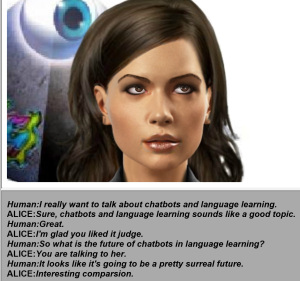
\includegraphics[width=10cm]{Pics/Chap1/alice.jpg}
  \caption{Một cuộc hội thoại giữa người thật và \alice{}.}
\end{figure}

Ta có thể thấy những câu trả lời của \alice{} tương đối phù hợp trong ngữ cảnh của cuộc hội thoại, không khác nhiều so với cách trả lời của người thật, tạo cảm giác như chatbot có thể hiểu được câu hỏi và trả lời một cách phù hợp. Tuy nhiên trong nhiều lĩnh vực ngày nay, chatbot không chỉ cần trong việc hỗ trợ tìm kiếm hay cung cấp thông tin cho người dùng, mà còn cần dùng cho những việc hoàn toàn tự động và có thể hiểu câu hỏi từ phía người dùng như đặt chỗ chuyến bay, đồ ăn ... hay điều khiển các thiết bị. Điều này dẫn đến một phương pháp khác trong việc xây dựng chatbot thực sự có trí thông minh, trí tuệ nhân tạo, đó là sử dụng \textit{Xử lý ngôn ngữ tự nhiên} (NLP - natural language processing) nhằm phân tích được cú pháp, ý nghĩa câu nói của người dùng đang hướng tới, hiểu rõ yêu cầu từ phía người dùng, để từ đó có thể đáp ứng những yêu cầu đó.

\subsection{Hệ thống trợ lý ảo}
Một \textit{trợ lý ảo} là một hệ thống phần mềm giúp thực hiện các nhiệm vụ hay các dịch vụ cho mỗi một cá nhân. Mỗi trợ lý ảo sẽ giúp cho người sử dụng thực hiện một nhiệm vụ trên một môi trường cụ thể như máy tính hay thiết bị điện thoại thông minh, hoặc trong chính căn nhà của mình để điều khiển các thiết bị nội thất trong ngôi nhà. Có nhiều phương thức để một trợ lý ảo có thể tương tác với người dùng như:

\begin{itemize}
	\item Văn bản (text)
	\item Âm thanh (voice)
	\item Ảnh được tải lên
\end{itemize}

Chatbot chính là một trợ lý ảo sử dụng văn bản hoặc giọng nói để cung cấp cho người dùng thông tin cần thiết hay chỉ đơn giản là trò chuyện với người dùng. Bên cạnh đó còn các trợ lý ảo được xây dựng để giúp người dùng thực hiện một nhiệm vụ nào đó như Google Assistant thông qua Google Allo có thể giúp người dùng tìm kiếm thông tin hay đặt lịch, giải trí và các nhiệm vụ cá nhân khác, hoặc thông qua Google Home để điều khiển các thiết bị thông minh trong ngôi nhà. Tại thời điểm hiện tại, các ông lớn trong ngành công nghệ như Google, Apple, Amazon hay Microsoft đã cho ra đời những trợ lý ảo của riêng mình và vẫn tiếp tục hoàn thiện để những trợ lý này trở thành một phần không thể thiếu trong cuộc sống hiện đại. Trong một bài viết trên trang Business Insider{\footnote{http://www.businessinsider.com/siri-vs-google-assistant-cortana-alexa-2016-11}} vào tháng 11/2016 đã đề cập đến một cuộc thi nhỏ giữa các trợ lý ảo của các ông lớn kể trên là Siri của Apple, Alexa của Amazon, Cortana của Microsoft và Google Assistant của Google. Kết quả được đánh giá dựa trên nhiều tiêu chí, mỗi trợ lý ảo đều có một điểm mạnh hay điểm yếu riêng trong những mục mà mình chưa hỗ trợ, tuy nhiên đánh giá chung là những trợ lý ảo này đều rất thông minh và có thể hiểu tối đa yêu cầu từ phía người dùng. 

\begin{figure}[H]
  \centering
    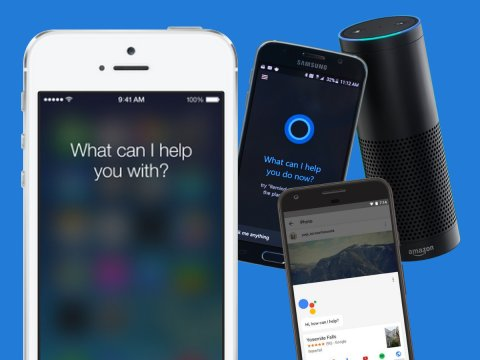
\includegraphics[width=10cm]{Pics/Chap1/virtual-assistants.png}
  \caption{Hình ảnh nền tảng của những trợ lý ảo nổi tiếng.}
\end{figure}

Những trợ lý ảo đang ngày càng phát triển cả về trí thông minh lẫn những lĩnh vực hiện hữu trong cuộc sống. Tuy nhiên những trợ lý ảo này mới chỉ phát triển trên ngôn ngữ là Tiếng Anh và hoàn toàn không có khả năng hiểu Tiếng Việt, gây ra cản trở trong mong muốn được tiếp cận những công nghệ tiên tiến trên thế giới của người Việt. Những trợ lý ảo đó có thể hiểu và phân tích được yêu cầu của người dùng bằng Tiếng Việt đã là một khó khăn, và sẽ khó khăn hơn nếu như người dùng sử dụng giọng nói để đưa yêu cầu vào hệ thống. Nhưng với sự hỗ trợ của những công ty lớn như Google trong việc nhận diện giọng nói Tiếng Việt và các nền tảng xây dựng chatbot sử dụng NLP, vấn đề này sẽ không còn bất khả thi nữa. Trong đề tài nghiên cứu này sẽ nêu rõ giải pháp để giải quyết vấn đề xây dựng chatbot để điều khiển điện thoại bằng giọng nói Tiếng Việt, và xa hơn nữa sẽ hỗ trợ để điều khiển các thiết bị trong ngôi nhà thông minh - Smart Home.

\section{Mục đích của đề tài}

Sự tiện dụng và những lợi ích mà chatbot hay những trợ lý ảo mang lại cho con người là vô cùng lớn, giúp cải thiện chất lượng cuộc sống của mọi người trong thời kì công nghệ đang ngày càng phát triển và trở thành một phần không thể thiếu trong đời sống. Ở Việt Nam hiện nay, những công nghệ thông minh cũng đang rất được quan tâm như điện thoại thông minh hay nhà thông minh. Bài viết vào đầu năm 2017{\footnote{http://baoquocte.vn/10-xu-huong-tieu-dung-cong-nghe-nam-2017-42757.html}} của \textit{baoquocte.vn} đã cho biết ``Trí tuệ nhân tạo (AI - Artificial Intelligence) sẽ là xu hướng nổi bật của năm 2017''. Trong bài viết đã nêu rõ sự có mặt khắp mọi nơi của trí tuệ nhân tạo, và có đến 35\% những người sử dụng Internet đều mong muốn có một cố vấn robot có trí tuệ nhân tạo để phục vụ những nhu cầu và lợi ích cá nhân. Bên cạnh đó, thời điểm này cũng đang là thời kì nở rộ của \textit{Internet of Things} - Vạn vật kết nối, khi mà các thiết bị điện tử dù lớn hay nhỏ trong gia đình hay trên các con phố cũng đều có thể kết nối với nhau trong một mạng Internet thống nhất và đều được kiểm soát chỉ thông qua một màn hình nhỏ của thiết bị thông minh như điện thoại hay máy tính bảng. Từ đó nhu cầu để điều khiển các thiết bị này không còn chỉ gói gọn ở trong việc sử dụng các thiết bị thông minh mà còn qua các phương thức khác nhau giọng nói, cử chỉ của tay chân hay thậm chí là sử dụng chính những suy nghĩ trong não bộ của con người.

Số lượng người sử dụng điện thoại thông minh ở Việt Nam cũng là rất cao, lên đến trên 25 triệu người trên tổng số trên 90 triệu dân và con số này sẽ còn tăng mạnh trong năm 2017 và những năm tiếp theo{\footnote{https://news.appota.com/bao-cao-thi-truong-mobile-viet-nam-q3-2016/}}. Cũng trong thời điểm này, có đến 39,8 triệu người Việt Nam sử dụng mạng Internet và khoảng 21,6 triệu người sử dụng Internet thông qua các thiết bị di động, điện thoại thông minh. Có thể thấy xu hướng sử dụng công nghệ ngày càng cao tại Việt Nam, và việc phát triển các sản phẩm trên các thiết bị này là một nhu cầu thiết yếu, đem lại nhiều lợi ích cho các doanh nghiệp Việt Nam nói riêng và nền kinh tế Việt Nam nói chung.

\begin{figure}[H]
  \centering
    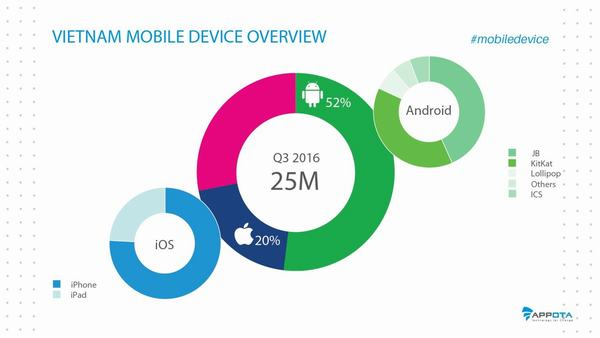
\includegraphics[width=15cm]{Pics/Chap1/mobile-vietnam.jpg}
  \caption{Tổng kết số lượng người sử dụng smart phone ở Việt Nam cuối năm 2016.}
\end{figure}

Với những người đang điều khiển các phương tiện giao thông như xe hơi thì việc sử dụng điện thoại thông minh và phải nhìn vào màn hình là một việc nguy hiểm, gây cản trở trong quá trình điều khiển xe, có thể gây ra tai nạn, hay khi sử dụng điện thoại mà người dùng phải thực hiện thao tác tay quá nhiều mới có thể hoàn thành được một nhiệm vụ hay yêu cầu sẽ gây ra cảm giác khó chịu, đặc biệt là việc nhập văn bản bằng tay trên các thiết bị di động thông minh rất khó khăn do bàn phím trên các thiết bị nhỏ, dễ gây nhầm lẫn khi nhập đoạn dài. Vì vậy trong đồ án nghiên cứu này sẽ đề xuất giải pháp để giải quyết cho vấn đề ``\textbf{Xây dựng chatbot điều khiển điện thoại bằng giọng nói Tiếng Việt}''. Đồ án sẽ tập trung vào việc xử lý giọng nói từ phía người dùng và chuyển thành dạng văn bản để có thể phân tích yêu cầu, từ đó xây dựng những tính năng giúp người dùng có thể điều khiển được chiếc điện thoại thông minh bằng chính giọng nói của mình với ngôn ngữ Tiếng Việt.

% Chapter 2
\chapter{Định hướng giải pháp}

Với vấn đề đã được đặt ra ở phần trên, đồ án đề xuất giải pháp với 2 mục tiêu chính là nhận diện giọng nói Tiếng Việt từ phía người dùng và xây dựng chatbot để phân tích yêu cầu từ phía người dùng (sử dụng \textit{Xử lý ngôn ngữ tự nhiên}).

\section{Nhận diện giọng nói}
\subsection{Khái niệm}
Nhận dạng giọng nói (Nhận dạng tiếng nói) là một quá trình \textit{nhận dạng mẫu}, với mục đích là phân lớp những thông tin đầu vào bằng giọng nói từ phía người dùng thành một chuỗi các kí tự (các từ) đã được học từ trước và lưu trữ lại trong bộ nhớ. Các mẫu là các đơn vị nhận dạng, có thể là một đoạn âm thanh của một từ hay một âm tiết. Nếu như việc nhận dạng chỉ dừng lại ở mức so sánh những mẫu có trong tập học với đoạn âm thanh và chọn ra mẫu trùng khớp nhất thì không có nhiều khó khăn. Những khó khăn cơ bản của nhận diện giọng nói có thể kể đến như:

\begin{itemize}
	\item Cùng là một từ hay một âm tiết cố định nhưng có vô vàn giọng nói khác nhau có thể diễn đạt lại được. Sự khác nhau đó là do âm lượng, tốc độ nói hay môi trường âm học của mỗi người là khác nhau, vì vậy khi chỉ sử dụng một giọng nói để làm mẫu nhận diện thì xác suất để nhận diện đúng và chính xác sẽ rất thấp, không mang lại nhiều giá trị nghiên cứu
	\item Thông thường người dùng sẽ không chỉ nói những câu nói bao gồm một từ đơn lẻ mà là một câu dài mang đủ ý nghĩa, kết hợp từ các từ đơn, từ ghép khác nhau. Việc phân tách được câu nói đó thành những chuỗi những cụm từ liên tục cũng là một việc làm khó khăn
	\item Tạp âm cũng là một phần gây nhiễu và khó khăn lớn trong việc nhận dạng giọng nói. Xác định những thông tin biến thiên nào là tiếng nói có ích và những thông tin nào là tiếng nói không có ích trong việc phân tích cũng là một yếu tố vô cùng quan trọng
\end{itemize}

\noindent Các nghiên cứu về nhận dạng tiếng nói dựa trên ba nguyên tắc cơ bản sau:
\begin{itemize}
	\item Tín hiệu tiếng nói được biểu diễn chính xác bởi các giá trị phổ trong một khoảng thời gian ngắn, nhờ vậy ta có thể trích ra các đặc điểm tiếng nói từ những khoảng thời gian ngắn và dùng các đặc điểm này để nhận dạng tiếng nói
	\item Nội dung của tiếng nói được biểu diễn dưới dạng chữ viết, là một dãy các ký hiệu ngữ âm, vì vậy ý nghĩa của một phát âm được bảo toàn khi chúng ta phiên âm phát âm thành các ký hiệu ngữ âm
	\item Nhận dạng tiếng nói là một quá trình nhận thức. Thông tin về ngữ nghĩa và suy đoán có giá trị trong quá trình nhận dạng tiếng nói, nhất là khi thông tin về âm học{\footnote{Âm học là một nhánh của vật lý học, nghiên cứu về sự lan truyền của sóng âm thanh trong các loại môi trường và sự tác động qua lại của nó với vật chất}} là không rõ ràng
\end{itemize}

Nhận diện giọng nói là một việc làm rất khó khăn từ việc xây dựng được bộ dữ liệu mẫu để so sánh đến việc xây dựng các mô hình thống kê xác suất để tổng quát hóa từ những mẫu tiếng nói thành những biến thiên quan trọng trong việc nhận dạng. Một số cách tiếp cận nhận dạng tiếng nói bằng thống kê bao gồm: mô hình Markov ẩn, mạng nơ-ron, sử dụng cơ sở tri thức \ldots.

\subsection{Google Speech Recognition API}
% .3cm
\subsubsection{Công cụ hỗ trợ nhận diện giọng nói}
Có rất nhiều các thư viện giúp nhận dạng giọng nói trên rất nhiều nền tảng, ngôn ngữ lập trình khác nhau và các ngôn ngữ của các quốc gia khác nhau, tuy nhiên với Tiếng Việt thì dường như không có nhiều vì để có thể nhận diện được thì cần một bộ dữ liệu mẫu vô cùng lớn mới có thể tăng độ chính xác lên được, và việc làm này gặp rất nhiều khó khăn ở Việt Nam do nguồn cung cấp giọng nói mẫu đầu vào không có. Cũng đã có những nhóm nghiên cứu nhận diện giọng nói Tiếng Việt ở Việt Nam, tuy nhiên chỉ dừng lại ở mức nhận diện một số những từ ngữ cụ thể để thực hiện một nhiệm vụ như ứng dụng iSago giúp cho người dùng chỉ việc nói tên của một quán phở hay một số tên loại món ăn khác, ứng dụng sẽ tìm kiếm và đưa ra gợi ý về những quán ăn gần đó, hay ứng dụng sử dụng giọng nói điều khiển xe lăn thông minh. Hầu hết các ứng dụng đều dừng lại ở mức nhận diện những từ đơn đơn giản và chưa có độ chính xác cao, cũng do một số nguyên nhân đã nêu ở trên.

Trên thế giới tại thời điểm hiện tại đã có một số những công ty lớn cung cấp thư viện hoặc thông qua API để hỗ trợ các lập trình viên tích hợp nhận diện giọng nói Tiếng Việt vào trong ứng dụng của mình. Có thể kể đến như:

\begin{itemize}
	\item Microsoft Speech Recognition SDK \footnote{Software development kit - Bộ công cụ phát triển phần mềm là một từ dùng để chỉ một tập những công cụ phát triển phần mềm mà cho phép việc tạo ra những ứng dụng bằng những gói phần mềm, nền tảng phần mềm, nền tảng phần cứng, hệ thống máy tính, hệ điều hành hay những nền tảng phát triển tương tự}
	\item Google Speech Recognition API
\end{itemize}
\noindent \textbf{Tại sao lại chọn Google Speech Recognition API?}\\[0.3cm]
\noindent Vào tháng 7/2013, Google đã công bố bộ ba công cụ tìm kiếm mới dành cho ngôn ngữ Tiếng Việt là Knowledge Graph (Sơ đồ Tri thức), Voice Search (Tìm kiếm bằng giọng nói) và Google Handwrite (Tìm kiếm bằng chữ viết tay). Theo bà Tamar Yehoshua, Giám đốc sản phẩm thuộc bộ phận Google Search, cho hay việc ``đào tạo'' công cụ tìm kiếm hiểu tiếng Việt là quá trình khó khăn: ``Chúng tôi cần hiểu cả người dùng lẫn nền văn hóa của Việt Nam. Chúng tôi có một đội ngũ chuyên về vấn đề này. Họ làm việc trực tiếp với người bản ngữ để thu thập các cách nói, cách phát âm... trong các điều kiện khác nhau như nhà hàng, trên phố đông hay bên trong xe hơi... Từ đó, họ xây dựng nhiều mẫu câu lệnh của những ngôn ngữ khác nhau để giúp hệ thống "học" cách nhận diện và hiểu ngôn ngữ''{\footnote{http://sohoa.vnexpress.net/tin-tuc/doi-song-so/google-ho-tro-tim-kiem-bang-giong-noi-tieng-viet-2842679.html}}. Và ngay sau đó, Google cũng đã cung cấp một bộ API{\footnote{API - Application program interface (giao diện chương trình ứng dụng là một tập các thủ tục, giao thức và công cụ cho việc xây dựng ứng dụng phần mềm}} hỗ trợ cho những lập trình viên mong muốn tích hợp nhận dạng giọng nói vào trong ứng dụng của mình có thể sử dụng hoàn toàn miễn phí.

Google là một công ty lớn với lượng người dùng truy cập hàng ngày từ khắp nơi trên thế giới là rất lớn, nên lượng dữ liệu từ tất cả các phương thức như văn bản hay giọng nói, chữ viết tay đều rất đa dạng và phong phú, chính vì vậy có đủ khả năng để tạo ra dữ liệu mẫu cho việc nhận dạng giọng nói. Không những thế, Google Speech Recognition cũng đã được tích hợp trên các thiết bị điện thoại thông minh chạy hệ điều hành Android từ 2.3 trở lên, rất thuận tiện cho những lập trình viên muốn phát triển ứng dụng trên nền tảng này.

\subsubsection{Tổng quan về Google Speech Recognition API}
\begin{formal}
	\begin{itemize}
		\item Nhà phát triển: Google
		\item Ra mắt lần đầu: 20/5/2002 (Google Voice Search)
		\item Phiên bản mới nhất: Hiện tại Google đã chuyển API lên Cloud chung của Google với phiên bản Google Cloud Speech API v1
		\item Tính năng nổi bật:
		\begin{itemize}
			\item Chuyển giọng nói thành văn bản (text)
			\item Sử dụng những mô hình mạng nơ-ron mạnh mẽ
			\item Nhận diện được hơn 80 ngôn ngữ của các quốc gia trên thế giới và những biến thể
			\item Nhận diện được thông qua những đoạn âm thanh được đưa vào trong request (yêu cầu được gửi lên từ phía server của người dùng)
			\item Trả lại kết quả dạng text với thời gian thực (real-time)
			\item Cơ chế loại bỏ tiếng ồn từ rất nhiều loại môi trường khác nhau
		\end{itemize}
	\end{itemize}
\end{formal}

Năm 2002, Google đã cho ra mắt Google Voice Action - là công cụ từ phòng nghiên cứu Google (Google Labs) cho phép mọi người sử dụng chiếc điện thoại của họ để thực hiện truy vấn bằng giọng nói tới Google. Người dùng sẽ phải gọi đến số (650) 623-6706, là số của hệ thống tìm kiếm bằng giọng nói của Google, sau đó họ phải đợi hệ thống phản hồi và nói ra từ khóa mà mình muốn tìm kiếm. Sau đó họ phải đợi trang web được cập nhật hoặc ấn vào một đường dẫn để dẫn đến trang kết quả tìm kiếm mà người dùng yêu cầu. Đến nay, những dịch vụ đó đã được dừng lại, thay vào đó, tìm kiếm bằng giọng nói đã được tích hợp sẵn vào trong các ứng dụng của Google như Google Maps, Google Mobile App \ldots

Hiện tại, Google Voice Action đã lấy tên là Google Voice Search hay Search by Voice là một sản phẩm của Google mà cho phép người dùng sử dụng tính năng Google Search bằng chính giọng nói của mình trên các thiết bị điện thoại thông minh hay máy vi tính. Và đến phiên bản hệ điều hành Android 4.1 trở lên, Google Voice Search đã được tích hợp vào trong Google Now. Tại thời điểm ban đầu, Google chỉ hỗ trợ nhận diện Tiếng Anh và những biến thể, sau đó lần lượt những ngôn ngữ của các quốc gia khác trên thế giới cũng được hỗ trợ, trong đó có Tiếng Việt.

\begin{figure}[H]
  \centering
    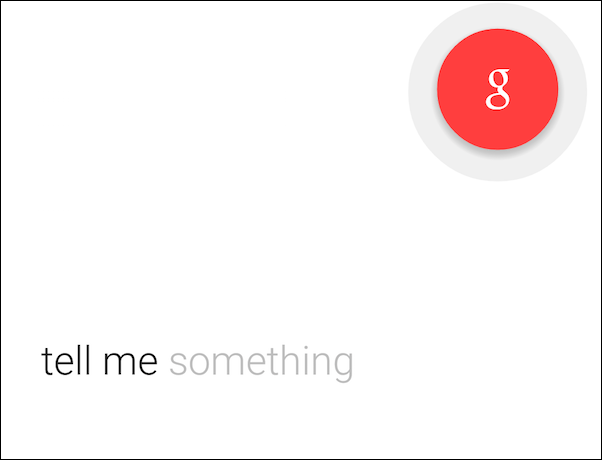
\includegraphics[width=10cm]{Pics/Chap2/google-voice.png}
  \caption{Giao diện chung của Google Voice Search.}
\end{figure}

Một đặc điểm quan trọng cần kể đến của Google Speech Recognition API chính là khả năng trả về kết quả thời gian thực, tức là kết quả được trả về với từng từ mà người dùng vừa nhập vào và chưa kết thúc câu nói của mình. Tính năng này giúp cho việc phát triển các ứng dụng trở nên dễ dàng và linh hoạt hơn, không cần đợi đến khi người dùng kết thúc nói mới trả về kết quả. Tính năng này cũng chính là một phần quan trọng giúp cho đồ án định hướng được những giải pháp hữu ích cho vấn đề cần giải quyết.

Tuy nhiên, sự sai sót trong việc nhận diện là không thể tránh khỏi do những nguyên nhân như môi trường xung quanh quá ồn dẫn đến âm lượng giọng nói của người dùng chưa đủ lớn, hay tốc độ nói của người dùng quá nhanh dẫn đến những nhập nhằng trong âm thanh. Vì vậy, trong đồ án đã nghiên cứu tìm ra phương pháp hạn chế lại những sai sót đó để có thể nắm bắt tốt nhất yêu cầu từ phía người dùng, đó là sử dụng một mô hình ngôn ngữ (Language Model) sẽ được giới thiệu chi tiết hơn ở phần sau của đồ án.

\section{Xây dựng chatbot}

Để xây dựng một chatbot cần phải xây dựng những thuộc tính hay hành vi của chatbot đó, những kiến thức mà sẽ giúp chúng phản ứng lại với những yêu cầu, đầu vào từ phía người dùng. Bên cạnh đó, để những chatbot đó có thể chạy được trên những nền tảng khác nhau, phục vụ cho những dịch vụ khác nhau như bán hàng hay cung cấp thông tin thì cần có sự hỗ trợ từ những bot platforms, để những chatbot có thể tương tác với người dùng qua nhiều kênh. Ta có một vài định nghĩa liên quan như sau:

\begin{itemize}
	\item Bot Platforms - nền tảng bot là những hệ sinh thái online (cung cấp dịch vụ qua mạng Internet), nơi mà những chatbot được triển khai và tương tác với người dùng, thực hiện những hành động mà chúng đã được cài đặt, hay thậm chí là tương tác với các nền tảng khác.
	\item Bot Development Frameworks - những bộ khung phát triển bot là nơi mà những chatbot sẽ được cài đặt và định nghĩa những hành vi của chúng. Một vài bộ khung phát triển bot có hỗ trợ xây dựng bot với khả năng xử lý ngôn ngữ tự nhiên
\end{itemize}

Chúng ta cần phân biệt được sự khác nhau giữa bot platforms và bot development frameworks. Hai khái niệm này có sự liên quan đến nhau nhưng việc phân biệt chúng cũng vô cùng quan trọng trong việc phát triển một hệ thống chatbot. Sự khác biệt lớn nhất là bot platform là nơi bot sống và tương tác với người dùng còn bot framework là nơi sinh ra các hành vi cho bot.

\subsection{Nền tảng chatbot}

Trên thế giới hiện nay, có rất nhiều nền tảng hay ứng dụng mà người dùng sử dụng để liên hệ, yêu cầu sự trợ giúp, hỗ trợ về mặt thông tin với các cửa hàng, các công ty cung cấp dịch vụ như Skype, Facebook Messenger, Slack \ldots Cửa hàng hay công ty nào cũng cần có những người nhân viên trực tổng đài hay hệ thống trả lời để sẵn sàng cung cấp cho khác hàng những thông tin cần thiết. Nhưng không phải lúc nào những nhân viên cũng sẵn sàng để cung cấp thông tin dù là lớn hay nhỏ, vì vậy các cửa hàng hay công ty dịch vụ đều muốn xây dựng riêng cho mình những chatbot có khả năng thay thế cho một hoặc nhiều nhân viên trực tổng đài, tăng khả năng chăm sóc khách hàng và lợi nhuận kinh doanh. Vậy làm thế nào để một chatbot của một cửa hàng, công ty cụ thể có thể được cài đặt trong những hệ thống của những ứng dụng liên lạc như Skype hay Facebook Messenger, để khi người dùng truy cập hay kết nối đến những chatbot đó, thông tin về cửa hàng, công ty mà chatbot đó đảm nhiệm sẽ được cung cấp phù hợp và chính xác cho người dùng. Bot platform chính là giải pháp cho vấn đề này.

Có rất nhiều những nền tảng hỗ trợ cho việc này, trên nhiều các ứng dụng liên lạc. Chúng ta có thể điểm qua một vài những nền tảng như vậy:

\begin{itemize}
	\item \textbf{ChattyPeople} là nền tảng chatbot tốt nhất trong việc tạo ra một chatbot có trí tuệ nhân tạo trên Facebook với khả năng tích hợp thương mại Facebook. Với ChattyPeople, chúng ta có thể tạo ra một chatbot Facebook Messenger nhanh chóng và dễ dàng, không cần yêu cầu về mặt coding. Sự đơn giản của nền tảng này làm cho nó phù hợp với những doanh nhân hay nhân viên môi giới ở trong những công ty nhỏ trong khi công nghệ mà nền tảng sử dụng lại phù hợp với lượng khách hàng lớn. Chúng ta hoàn toàn có thể tạo ra được những hệ thống chăm sóc và trả lời khách hàng hoặc tích hợp chúng vào trong Facebook Messenger.

	\begin{figure}[H]
	  \centering
	    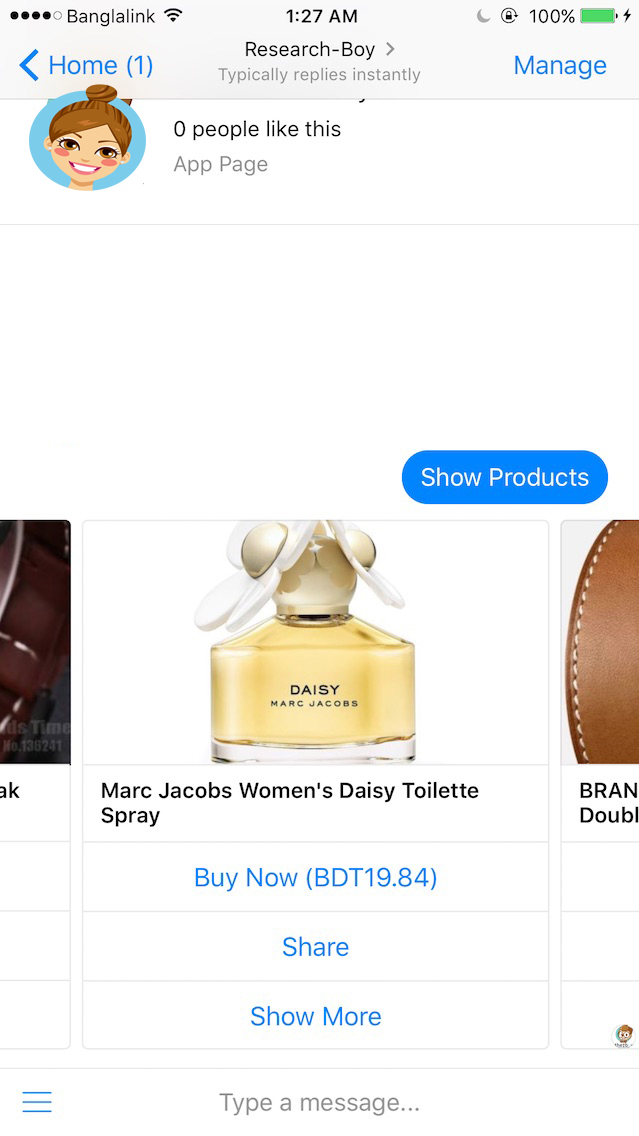
\includegraphics[width=7cm]{Pics/Chap2/chatty-prople.jpg}
	  \caption{Một ví dụ trong gợi ý sản phẩm của ChattyPeople bot.}
	\end{figure}

Ngoài ChattyPeople còn có một vài nền tảng khác như \textit{MEOKAY} hay \textit{Botsify}, \textit{Chatfuel} cũng hỗ trợ xây dựng và triển khai các chatbot trên Facebook Messenger.

	\item \textbf{BotKit} là một bộ công cụ giúp xây dựng một chatbot trên Facebook Messenger, Slack, Twilio và những ứng dụng tin nhắn khác. BotKit có thể được sử dụng để tạo ra những ứng dụng thông minh có khả năng hội thoại như một người thật. Tính chất này đã mang lại điểm khác biệt cho BotKit so với những nền tảng hỗ trợ triển khai chatbot khác.

	\item \textbf{FlowXO} là một nền tảng hỗ trợ triển khai bot khác cho việc kinh doanh trên Facebook Messenger, Slack, SMS, Telegraph \ldots Nền tảng này cho phép tạo ra rất nhiều tính linh hoạt khác nhau trong bot bằng cách cài đặt các lựa chọn để tạo ra những chatbot hoàn toàn tự động hay có thể tích hợp vào các hệ thống khác.
\end{itemize}

Còn rất nhiều các nền tảng hỗ trợ trong việc triển khai chatbot trong việc kinh doanh cũng như các dịch vụ doanh nghiệp khác tại thời điểm hiện tại. Tuy nhiên đồ án được triển khai trên ứng dụng của thiết bị điện thoại thông minh nên việc sử dụng một nền tảng là chưa cần thiết. Có một vài nền tảng ngoài hỗ trợ triển khai còn hỗ trợ việc xây dựng trí thông minh cho chatbot như API.AI hay Beep Boop, tuy nhiên ngoài việc mất phí thì việc làm này cũng là chưa cần thiết đối với giải pháp mà đồ án hướng tới. Để phân tích được yêu cầu từ phía người dùng, đồ án đề xuất sử dụng một bot framework để giải quyết vấn đề này.

\subsection{Framework phát triển bot} \label{subsec:frameworkchatbot}

Chatbot như đã nêu ở trên là một phần mềm cho phép tạo ra những cuộc hội thoại mà người dùng có cảm giác như đang được nói chuyện với một người thật. Những chatbot đơn giản sử dụng công thức chung là pattern-matching, so sánh những dữ liệu đầu vào với một tập các câu nói có sẵn trong tập dữ liệu học và chọn ra câu trả lời phù hợp nhất. Tuy nhiên với những dịch vụ muốn hiểu rõ hơn yêu cầu từ phía người dùng và đưa ra câu trả lời có nhiều ý nghĩa hơn thì những chatbot như trên chưa thể giải quyết được. Hiện tại đã có rất nhiều những thư viện được xây dựng nhằm hỗ trợ phát triển những chatbot sử dụng xử lý ngôn ngữ tự nhiên. Việc làm này là khó khăn hơn rất nhiều so với những chatbot thông thường do phải phân tách được cấu trúc câu nói người dùng và lấy được những thông tin quan trọng trong câu nói đó. Tiếng Anh thường là ngôn ngữ đầu tiên mà những thư viện này hướng tới, có thể kể đến một vài thư viện nổi tiếng như:

\begin{itemize}
	\item Với \textit{API AI}, chúng ta có thể xây dựng những chatbot, ứng dụng hay dịch vụ với sự tương tác ngôn ngữ tự nhiên hoàn toàn riêng biệt. Có thể nói API AI là nền tảng NLU - Natural Language Understanding hoàn thiện nhất trên thị trường. API AI cho phép người dùng truy cập thông qua SMS, âm thanh hay văn bản (chat). Bên cạnh đó, API AI còn hỗ trợ giao diện vô cùng linh hoạt và dễ dàng cho người sử dụng, với những tính năng mạnh mẽ cho việc phát triển những hệ thống câu hỏi - trả lời phức tạp. Tổng kết lại, API AI có đầy đủ tất cả bao gồm: giải pháp hoàn thiện, Học máy, Hỗ trợ hội thoại, tích hợp, dễ dàng triển khai, đa nền tảng và đa ngôn ngữ. Tuy nhiên API AI lại không thể hỗ trợ trong đề tài do không hỗ trợ Tiếng Việt
	\item \textit{Microsoft LUIS} là một framework hỗ trợ xây dựng chatbot rất mạnh được phát triển bởi Microsoft, tiện lợi cho việc kết hợp với Microsoft Bot Builder là một nền tảng hỗ trợ triển khai chatbot. LUIS có giao diện khá đơn giản và dễ sử dụng. Mục tiêu chính của LUIS mà người dùng cần hướng tới là xây dựng một bộ những intent - là những ý định, dự định mà người dùng muốn hướng tới. Ví dụ người dùng muốn bắt các trường hợp về việc chào hỏi thì họ sẽ tạo ra intent tên là greeting. Trong intent này, người dùng sẽ cung cấp những câu nói mà người dùng cho là sẽ nằm trong trường hợp chào hỏi như ``Xin chào'' hay ``Chào bạn, bạn thế nào?''. Dựa vào tập huấn luyện và khả năng xử lý ngôn ngữ tự nhiên, với những câu nói mới chưa từng có hoặc tương tự với những câu đã có trong cơ sở dữ liệu, LUIS sẽ đánh giá xác suất khả năng mỗi câu được phân loại vào các intent và chọn ra intent mà có xác suất câu đó nằm trong lớn nhất. Bên cạnh đó, người dùng cũng cần xây dựng những entity để giúp cho việc nhận diện được chính xác hơn. Với câu nói ``Hôm nay là ngày bao nhiêu?'' hay ``Ngày mai là thứ mấy?'', những từ như ``Hôm nay'' hay ``Ngày mai'' sẽ được LUIS nhận dạng vào một entity đã xây dựng sẵn, phục vụ cho việc phân biệt khoảng thời gian người dùng nhắc tới, từ đó người dùng sẽ đưa ra những xử lý của chatbot một cách hợp lý cho mỗi trường hợp. Tuy nhiên trên hết, LUIS cũng chưa hỗ trợ Tiếng Việt nên cũng không thể áp dụng cho đề tài
\end{itemize}

Với khả năng hỗ trợ ngôn ngữ Tiếng Việt, là một công cụ trong việc phân tích câu nói sử dụng xử lý ngôn ngữ tự nhiên được Facebook Messenger Framework lấy làm tiêu chuẩn, \textbf{Wit.ai} là một lựa chọn phù hợp với mục đích và hướng giải quyết vấn đề của đề tài. Cũng tương tự LUIS, Wit.ai cũng xây dựng bộ dữ liệu học dựa trên phân tách câu nói từ phía người dùng thành các entity, bao gồm built-in entity là những entity đã được xây dựng sẵn và những user entity là những entity do người dùng tự định nghĩa ra. Tuy với Tiếng Việt, những built-in entity chưa có nhiều loại như đối với Tiếng Anh nhưng việc nhận dạng với những câu mới và có ý diễn đạt tương tự câu đã huấn luyện là rất chính xác. Framework này sẽ được nói rõ hơn ở những phần sau của báo cáo.

\section{Công cụ hỗ trợ quá trình phát triển}
Để xây dựng hệ thống cho đề tài nghiên cứu, em đã sử dụng một số công cụ nhằm hỗ trợ việc quản lý mã nguồn, phiên bản và tiến độ của dự án như:
\begin{itemize}
	\item \textbf{Git}: là công cụ quản lý mã nguồn và phiên bản hiệu quả, giúp cho việc phát triển các tính năng của sản phẩm nhanh hơn và rõ ràng hơn.
	\item \textbf{Trello}: Liệt kê toàn bộ những công việc cần làm và thời gian cần hoàn thành, bên cạnh đó cũng là những bình luận ghi lại những điều đã tìm hiểu được trong quá trình nghiên cứu.
\end{itemize}

\stopcontents[parts]

\part{Các kết quả đạt được}
\startcontents[parts]
\printcontents[parts]{}{-1}{\setcounter{tocdepth}{1}}

% Chapter 3
\chapter{Tổng quan}
\section{Mô hình hệ thống}
Đồ án đề xuất mô hình hệ thống để giải quyết vấn đề đã được nêu ở phần trên:

\begin{figure}[H] \label{fig:VVC}
	\centering
		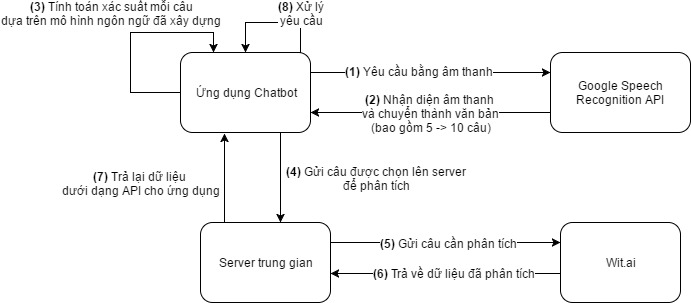
\includegraphics[width=15cm]{Pics/Chap2/VVC.jpg}
	\caption{Mô hình hệ thống.}
\end{figure}

\noindent Trong đó có các thành phần chính sau:

\begin{itemize}
	\item \textbf{Ứng dụng chatbot} là ứng dụng được xây dựng trên điện thoại thông minh chạy hệ điều hành Android, là thành phần chính giao tiếp với người dùng
	\item \textbf{Google Speech Recognition API} là dịch vụ giúp phân tích giọng nói thành dạng văn bản
	\item \textbf{Wit.ai} framework hỗ trợ huấn luyện khả năng thông minh cho chatbot
	\item \textbf{Server trung gian} là dịch vụ trung gian xử lý các trường hợp được nhận diện từ phía Wit.ai và trả về các kết quả tương ứng cho ứng dụng
\end{itemize}

\noindent Với mô hình hệ thống đề xuất, có 8 bước chính được thực hiện:

\begin{enumerate}
	\item Sử dụng thư viện có sẵn được tích hợp trong hệ điều hành Android để gửi luồng (stream) dữ liệu âm thành từ phía lên Google Speech Recognition API xử lý và trả về kết quả
	\item Nhận kết quả trả về từ phía Google là một tập các câu có cách phát âm tương tự nhau do cách phát âm, âm lượng, ngữ âm của người dùng làm cho Google Speech Recognition API có sự nhập nhằng và không chắc chắn
	\item Thông thường, kết quả đầu tiên trong tập dữ liệu trả về là kết quả chính xác nhất mà Google phân tích được. Tuy nhiên, do những nguyên nhân về âm thanh, kết quả chính xác nhất có thể không nằm ở kết quả đầu tiên hoặc không có kết quả nào trùng khớp với lời nói của người dùng. Hệ thống đề xuất sử dụng phương pháp \textit{Mô hình ngôn ngữ} để tính xác suất xảy ra của mỗi câu dựa vào một tập dữ liệu học đã được xây dựng từ trước, từ đó chọn ra câu có xác suất xảy ra cao nhất để mang đi phân tích yêu cầu
	\item Ứng dụng chatbot gửi câu lệnh là kết quả đã được chọn ra ở bước trên lên phía server trung gian
	\item Server trung gian gửi câu lệnh lên cho Wit.ai
	\item Wit.ai trả về API chứa những dữ liệu đã được phân tích từ câu lệnh
	\item Server trung gian chọn lọc ra những thông tin cần thiết từ phía Wit.ai và trả dữ liệu đã chọn lọc về cho ứng dụng
	\item Với những kết quả đã phân tích, ứng dụng thực hiện hành động phù hợp với yêu cầu từ phía người dùng
\end{enumerate}

\section{Các yêu cầu về chức năng} \label{sec:requirement}
\begin{itemize}
	\item Xây dựng hệ thống thành một thư viện Android, có thể tích hợp vào những ứng dụng điều khiển hệ thống bằng giọng nói Tiếng Việt
	\item Hỗ trợ điều khiển điện thoại với các tính năng
	\begin{itemize}
		\item Mở ứng dụng
		\item Bật/tắt đèn, bluetooth, mạng ...
		\item Đặt lịch hẹn, đồng hồ báo thức
		\item Tìm kiếm thông tin
	\end{itemize}
	\item Có khả năng trả lời những câu nói thông thường của người dùng mà không phải là yêu cầu điều khiển
\end{itemize}

\section{Các yêu cầu phi chức năng}
\begin{itemize}
	\item Chọn ra câu nói chính xác trong tập dữ liệu trả về từ phía Google Speech Recognition API với độ chính xác là 85\%
	\item Ứng dụng chạy ổn định, phản hồi người dùng sau tối đa 2 giây
\end{itemize}

% Chapter 4
\chapter{Cơ sở lý thuyết}
\section{Mô hình ngôn ngữ}
\subsection{Khái niệm}
Mô hình ngôn ngữ (LM - Language Model) thống kê cho phép ước lượng xác suất của một chuỗi m phần tử $P(w_1 w_2 \ldots w_m)$ (ở đây $w_1$, $w_2$ \ldots  là các từ trong câu cần tính xác suất), tức là khả năng của một chuỗi từ có thể xuất hiện trong một ngôn ngữ. Theo công thức Bayes, ta có:
\[P(AB)=P(A|B)*P(A)\]

Từ đó ta có được công thức:
\begin{align*}
	P(w_1w_2 \ldots w_m) &= P(w_m|w_1w_2 \ldots w_{m-1}) \\
						&= \ldots \\
						&= P(w_1)*P(w_2|w_1)* \ldots *P(w_m|w_1w_2 \ldots w_{m-1})
\end{align*}

Theo công thức Bayes, mô hình ngôn ngữ cần phải có một lượng bộ nhớ vô cùng lớn để có thể lưu hết được xác suất của tất cả các chuỗi độ dài nhỏ hơn m để qua đó có thể thống kê và tính xác suất cho từng thành phần nhỏ, sau đó mới đem nhân lại với nhau để ra được xác suất cuối cùng của cả câu. Trên thực tế, việc làm này là không thể do độ dài của một câu có thể là vô hạn, độ dài của m có thể tiến ra vô cùng. Tuy nhiên giả thuyết Markov giúp giải quyết vấn đề này.
Để giải quyết vấn đề này, ta có thể sử dụng xấp xỉ Markov bậc n. Ta có:
\[P(w_m|w_1w_2 \ldots w_{m-1}) \approx P(w_m|w_{m-n}w_{m-n+1} \ldots w_{m-1})\]

Tức là, với xấp xỉ Markov, xác suất xảy ra của một từ $w_m$ trong câu chỉ phụ thuộc vào n từ đứng đằng trước nó, thay vì việc tính $P(w_m|w_1*w_2 \ldots w_{m-1})$, ta chỉ cần tính $P(w_m|w_{m-n} \ldots w_{m-1})$. Áp dụng công thức trên, ta có thể viết lại công thức tính xác suất cho một câu có m từ:
\begin{equation} \label{eq:markov}
	\begin{aligned} 
	P(w_1w_2 \ldots w_m) &= P(w_1)*P(w_2|w_1)* \ldots *P(w_m|w_{m-n}w_{m-n+1} \ldots w_{m-1}) \\
						&= \prod_{i}{P(w_i|w_{i-n} \ldots w_{i-1})}
	\end{aligned}
\end{equation}

Với công thức trên, ta hoàn toàn có thể xây dựng một mô hình ngôn ngữ thống kê toàn bộ những cụm từ có độ dài nhỏ hơn hoặc bằng \textit{n} từ. Một mô hình ngôn ngữ như vậy sẽ được gọi là mô hình \texttt{N-gram} trong đó \textit{N} là độ dài tối đa của một cụm được thống kê trong mô hình ngôn ngữ đó. Ta có một ví dụ như sau:

\begin{formal} 
Cho một tập các câu nói:
	\begin{itemize}
		\item <s> tôi muốn bật đèn </s>
		\item <s> hãy bật đèn lên giúp tôi </s>
		\item <s> tôi muốn bật điều hòa </s>
		\item <s> giúp tôi mở tivi </s>
	\end{itemize} 
Tính xác suất xảy ra của các câu trên theo mô hình ngôn ngữ \texttt{N-gram}
\label{fm:ex}
\end{formal}

Trong các ví dụ trên có sử dụng ``<s>'' và ``</s>'' là kí tự đánh dấu bắt đầu và kết thúc câu. Giả sử ta đã huấn luyện được một mô hình ngôn ngữ \texttt{N-gram} (việc huấn luyện sẽ được giới thiệu ở phần sau), ta muốn tính xác suất xảy ra của các câu trong ví dụ trên, ta cần dùng đến công thức \ref{eq:markov}. Với câu ``tôi muốn bật đèn'', ta có thể tính với:

\begin{itemize}
	\item \texttt{N = 1} - Unigram: Tính xác suất của một từ mà không phụ thuộc vào các từ đứng trước
		\[P(\text{Tôi muốn bật đèn}) = P(\text{tôi}) * P(\text{muốn}) * P(\text{bật}) * P(\text{đèn})\]
	\item \texttt{N = 2} - Bigram: Tính xác suất của một từ phụ thuộc vào một từ đứng trước
		\[P(\text{tôi muốn bật đèn}) = P(\text{tôi}) * P(\text{muốn}|\text{tôi}) * P(\text{bật}|\text{muốn}) * P(\text{đèn}|\text{bật})\]
	\item \texttt{N = 3} - Trigram: Tính xác suất của một từ phụ thuộc vào hai từ đứng trước
		\[P(\text{tôi muốn bật đèn}) = P(\text{tôi}) * P(\text{muốn}|\text{tôi}) * P(\text{bật}|\text{tôi muốn}) * P(\text{đèn}|\text{muốn bật})\]
\end{itemize}

Ta lại có việc tính phép nhân bao giờ cũng mất thời gian hơn việc tính phép cộng, vì vậy để giảm thời gian tính xác suất của mỗi câu, thay vì việc tính phép nhân các xác suất, ta tính tổng logarit cơ số 10 của các xác suất. Ta có:
\[\log(p_1*p_2* \ldots p_m) = \log(p_1) + \log(p_2) + \ldots + \log(p_m)\]

Vậy với ví dụ câu ``tôi muốn bật đèn'', thay vì việc tính tích xác suất như trên, ta có thể tính logarit của nó. Cụ thể là (ví dụ với N = 1):
\[\log(P(\text{tôi muốn bật đèn})) = \log(P(\text{tôi})) + \log(P(\text{muốn})) + \ldots + \log(P(\text{đèn}))\]

Tương tự với các trường hợp N = 2, N = 3, \ldots Ta sử dụng logarit để so sánh giữa các câu. Câu nào có hệ số logarit càng lớn thì câu đó xác suất xảy ra càng lớn. Vậy để tính xác suất từng phần của tích các xác suất, ta có thể làm như thế nào?

Theo lý thuyết \textit{Ước lượng khả năng tối đa} (Maximum Likelihood Estimate - MLE), gọi $C(w_1w_2 \ldots w_m)$  là tần suất xuất hiện của cụm $w_1w_2 \ldots w_m$ trong tập huấn luyện mô hình ngôn ngữ, ta có công thức:

\[P(w_m|w_{m-n}w_{m-n+1} \ldots w_{m-1}) = \frac{C(w_{m-n}w_{m-n+1} \ldots w_m)}{C(w_{m-n}w_{m-n+1} \ldots w_{m-1})}\]

Công thức trên còn gọi là công thức tính xác suất ``thô''. Với công thức trên, khi một câu chứa một cụm từ chưa từng xuất hiện trong tập huấn luyện thì mặc nhiên tần suất xuất hiện của cụm từ đó sẽ bằng 0, từ đó dẫn đến xác suất của toàn bộ cả câu cũng sẽ bằng 0, gây ra sự sai sót. Có thể ví dụ đến trường hợp bigram (N=2), mỗi một bigram được tạo ra từ 2 unigram (N=1) bất kì, vì vậy với một tập học có $m$ cụm unigram riêng biệt thì có thể có đến $m^2$ cụm bigram có thể có. Tuy nhiên trong tập huấn luyện sẽ không thể chứa đủ từng đó cụm bigram, vì vậy khi đưa một câu bất kì vào để tính xác suất sẽ xuất hiện những cụm bigram chưa từng xuất hiện lần nào trong tập huấn luyện mô hình ngôn ngữ. Để tránh tình trạng này, người ta đã đưa ra các phương pháp ``làm mịn''.

Ta cũng cần nói thêm về việc huấn luyện một mô hình ngôn ngữ, tức là từ một tập các câu nói, câu văn chính xác (như ở ví dụ \ref{fm:ex}) về ngữ pháp và cấu trúc câu, ta sẽ tìm cách để ước lượng xác suất xảy ra của một câu văn chưa biết trong tương lai (có thể là một câu trong tập kiểm thử hoặc một câu nói bất kì) xem độ phù hợp của câu văn đó đối với tập huấn luyện là như thế nào. Ta có ví dụ với 2 câu nói như sau:

\begin{itemize}
 	\item tôi muốn bật đèn
 	\item tôi giúp ban đêm
 \end{itemize} 

2 câu nói này hoàn toàn có thể là một ví dụ cho kết quả trả về trong việc nhận diện giọng nói từ phía Google Speech Recognition API trong sự nhập nhằng do âm thanh của người dùng gây ra, vì vậy để lựa chọn được chính xác câu nói phù hợp, ta tính xác suất của 2 câu nói này dựa vào tập huấn luyện theo ví dụ \ref{fm:ex} với N lần lượt là 1, 2, 3. Ta có kết quả sau:

\begin{table}[h]
	\caption{Xác suất của 2 câu nói trong ví dụ}
	\centering
	\begin{tabular}{ | c | C | C | C | }
	\hline
	Câu nói & N = 1 & N = 2 & N = 3 \\
	\hline
	tôi muốn bật đèn & $0,36.10^{-3}$ & 0.0417 & 0.25  \\
	\hline
	tôi giúp ban đêm & 0 & 0 & 0  \\
	\hline
	\end{tabular}
\end{table}

Dễ dàng thấy được câu ``tôi muốn bật đèn'' có xác suất xảy ra cao hơn so với câu ``tôi giúp ban đêm'', vì vậy ta sẽ lựa chọn câu ``tôi muốn bật đèn''. Tuy nhiên, tại sao tất cả xác suất của câu ``tôi giúp ban đêm'' lại đều bằng 0, đơn giản là do trong câu đó có cụm từ chưa từng xuất hiện trong tập huấn luyện, dẫn đến xác suất của cụm từ đó bằng 0, và khi đem nhân với xác suất của các cụm từ khác dù khác 0 thì vẫn cho ra kết quả tích xác suất cuối cùng là bằng 0. Việc này sẽ gây ảnh hưởng nhiều đến việc chọn lựa do đó hoàn toàn có thể là một câu nói nhận diện chính xác từ giọng nói của người dùng nhưng do có chứa cụm từ không tồn tại trong tập huấn luyện mà xác suất bị bằng 0. Để giải quyết cho vấn đề này, chúng ta sử dụng các phương pháp \textit{``làm mịn''}.

\subsection{Các phương pháp làm mịn}

Nguyên lý chung của các phương pháp ``làm mịn'' là:

\begin{itemize}
	\item Gán cho các cụm n-gram có xác suất bằng 0 (chưa từng xuất hiện trong tập huấn luyện) một giá trị khác 0
	\item Thay đổi lại giá trị xác suất của các cụm n-gram có xác suất khác 0 thành một giá trị phù hợp (tổng xác suất của tất cả các khả năng n-gram khác nhau phải đảm bảo không đổi, bằng 100\%)
\end{itemize}

\noindent Từ đó ta có các loại phương pháp làm mịn như sau:

\begin{itemize}
	\item \textit{Chiết khấu} (Discouting): giảm lượng nhỏ xác suất của các cụm n-gram có xác suất lớn hơn 0 để bù cho các cụm n-gram không xuất hiện trong tập huấn luyện. Điển hình là các phương pháp: Add-one, Witten-Bell và Good-Turing
	\item \textit{Truy hồi} (Back-off): tính toán xác suất của cụm n-gram không xuất hiện trong tập huấn luyện dựa vào các cụm n-gram thành phần có độ dài ngắn hơn và có xác suất khác 0
	\item \textit{Nội suy} (Interpolation): tính toán xác suất của tất cả các cụm n-gram dựa vào xác suất của các cụm n-gram ngắn hơn
\end{itemize}

Mỗi phương pháp làm mịn đều mang lại những lợi ích khác nhau, tuy nhiên việc đánh giá phương pháp nào phù hợp với hệ thống sẽ được trình bày ở phần \ref{chap:setup}.

\section{Xử lý ngôn ngữ tự nhiên}

\subsection{Khái niệm}

\textbf{Xử lý ngôn ngữ tự nhiên} là một nhánh của khoa học máy tính, trí tuệ nhân tạo và ngôn ngữ máy tính, quan tâm đến sự tương tác giữa máy tính và ngôn ngữ tự nhiên của con người, hay chi tiết hơn là lập trình máy tính để xử lý hiệu quả nhất một lượng lớn những thể hiện của ngôn ngữ tự nhiên. Những thách thức trong xử lý ngôn ngữ tự nhiên thông thường liên quan đến \textit{hiểu ngôn ngữ tự nhiên} (Natural Language Understanding), \textit{sinh ngôn ngữ tự nhiên} (Natural Language Generation) \ldots

Đối với mỗi ngôn ngữ đều có những đặc thù về cách xử lý riêng, tuy nhiên có một số bước xử lý chung như sau:

\begin{itemize}
	\item \textit{Phân tích hình thái} - Trong bước này từng từ sẽ được phân tích và các ký tự không phải chữ (như các dấu câu) sẽ được tách ra khỏi các từ. Trong tiếng Anh và nhiều ngôn ngữ khác, các từ được phân tách với nhau bằng dấu cách. Tuy nhiên trong tiếng Việt, dấu cách được dùng để phân tách các tiếng (âm tiết) chứ không phải từ và đây là một công việc không hề đơn giản.
	\item \textit{Phân tích cú pháp} - Dãy các từ sẽ được biến đổi thành các cấu trúc thể hiện sự liên kết giữa các từ này. Sẽ có những dãy từ bị loại do vi phạm các luật văn phạm.
	\item \textit{Phân tích ngữ nghĩa} - Thêm ngữ nghĩa vào các cấu trúc được tạo ra bởi bộ phân tích cú pháp.
	\item \textit{Tích hợp văn bản} - Ngữ nghĩa của một câu riêng biệt có thể phụ thuộc vào những câu đứng trước, đồng thời nó cũng có thể ảnh hưởng đến các câu phía sau.
	\item \textit{Phân tích thực nghĩa} - Cấu trúc thể hiện điều được phát ngôn sẽ được thông dịch lại để xác định nó thật sự có nghĩa là gì.
\end{itemize}

Bên cạnh đó là các bài toán và ứng dụng liên quan đến xử lý ngôn ngữ tự nhiên như:

\begin{itemize}
	\item \textit{Nhận dạng chữ viết}: Có hai kiểu nhận dạng, thứ nhất là nhận dạng chữ in, ví dụ nhận dạng chữ trên sách giáo khoa rồi chuyển nó thành dạng văn bản điện tử hoặc phức tạp hơn là nhận dạng chữ viết tay, có khó khăn bởi vì chữ viết tay không có khuôn dạng rõ ràng và thay đổi từ người này sang người khác. Với chương trình nhận dạng chữ viết in có thể chuyển hàng ngàn đầu sách trong thư viện thành văn bản điện tử trong thời gian ngắn. Nhận dạng chữ viết của con người có ứng dụng trong khoa học hình sự và bảo mật thông tin (nhận dạng chữ ký điện tử).
	\item \textit{Nhận dạng tiếng nói}: Nhận dạng tiếng nói rồi chuyển chúng thành văn bản tương ứng. Giúp thao tác của con người trên các thiết bị nhanh hơn và đơn giản hơn, chẳng hạn thay vì gõ một tài liệu nào đó bạn đọc nó lên và trình soạn thảo sẽ tự ghi nó ra. Đây cũng là bước đầu tiên cần phải thực hiện trong ước mơ thực hiện giao tiếp giữa con người với robot. Nhận dạng tiếng nói có khả năng trợ giúp người khiếm thị rất nhiều.
	\item \textit{Tổng hợp tiếng nói}: Từ một văn bản tự động tổng hợp thành tiếng nói. Thay vì phải tự đọc một cuốn sách hay nội dung một trang web, nó tự động đọc cho chúng ta. Giống như nhận dạng tiếng nói, tổng hợp tiếng nói là sự trợ giúp tốt cho người khiếm thị, nhưng ngược lại nó là bước cuối cùng trong giao tiếp giữa robot với người.
	\item \textit{Tóm tắt văn bản}: Từ một văn bản dài tóm tắt thành một văn bản ngắn hơn theo mong muốn nhưng vẫn chứa những nội dung thiết yếu nhất. Đây cũng là một ứng dụng cần thiết trong việc nắm bắt nội dung từ câu nói của người dùng.
\end{itemize}

Còn một số bài toán khác trong lĩnh vực xử lý ngôn ngữ tự nhiên. Tuy nhiên trong đề tài này, ta cần quan tâm đến xử lý tự nhiên trong ứng dụng chatbot.

\subsection{Xử lý ngôn ngữ tự nhiên trong chatbot}

Chìa khóa cho một chatbot có thể hiểu được con người là khả năng hiểu được mong muốn, dự định - \textbf{intent} của con người và trích xuất ra được những thông tin liên quan với dự định đó, cùng với những hành động xử lý liên quan.

Vì vậy, trong lĩnh vực xây dựng chatbot sử dụng xử lý ngôn ngữ tự nhiên, chúng ta sẽ quan tâm đến khía cạnh làm sao để một chatbot có thể nắm bắt được ý định, mong muốn của người dùng qua một câu nói và trích xuất ra được những thông tin liên quan, quan trọng nằm trong câu nói đó của người dùng. \\[0.3cm]
\noindent \textbf{Vậy làm thế nào để dự đoán và trích xuất thông tin?\\[0.3cm]}
Một hệ thống xử lý ngôn ngữ tự nhiên được sử dụng trong chatbot sẽ không tìm kiếm những từ khóa nằm trong câu nói, văn bản như một bộ máy tìm kiếm mà thay vào đó là việc sử dụng những kiến thức mà hệ thống đã được học thông qua các cấu trúc câu, thuật ngữ và khả năng nhận diện những mẫu đã được học để cố gắng tính toán và ghép câu nói của người dùng vào một tình huống intent đã được xây dựng từ trước. Có nghĩa là, chatbot sẽ được lập trình để nhận diện những thứ chắc chắn mà mọi người muốn và phản hồi lại. Có 4 lĩnh vực con cần nhắc tới trong xử lý ngôn ngữ tự nhiên áp dụng cho chatbot:

\begin{itemize}
	\item \textbf{Những hệ thống hội thoại}
	Một chatbot cần có một giao diện với người dùng. Trong thực tế, khi con người giao tiếp với nhau, chúng ta sử dụng rất nhiều các giác quan để cảm nhận như tai để nghe, mắt để thấy, hay sử dụng xúc giác để cảm nhận. Vì vậy một cuộc đối thoại sẽ được cảm nhận đầy đủ và rõ nét nhất. Tuy nhiên, khi người nói chuyện với người còn nhiều khi có những sự hiểu nhầm, chứ không nói đến việc chatbot chỉ tương tác trực tiếp với người dùng thông qua văn bản. Việc đó không khác nào sự tương tác giữa người với người thông qua các ô chatbox của các trang mạng xã hội. Để biểu đạt được cảm xúc của mình, người ta sẽ cần dùng tới những avatar là những biểu tượng thay thế cho khuôn mặt, thể hiện cảm xúc hiện tại của bản thân mình cho người khác biết. Và khi đó, với một chatbot, chúng ta hoàn toàn có thể xây dựng để chatbot thông minh hơn và hiểu cảm xúc của người dùng hơn thông qua các avatar cảm xúc
	\item \textbf{Hiểu ngôn ngữ tự nhiên}
	Một việc rất khó khăn trong xử lý ngôn ngữ tự nhiên là phân loại hình thái của từ trong câu. Ví dụ như từ ``bay'' trong tiếng Việt hoàn toàn có thể là một động từ chỉ một hành động của loài chim, nhưng cũng hoàn toàn có thể là một danh từ chỉ một vật dụng trong xây dựng là ``cái bay''. Vì vậy một chatbot thực sự thông minh cần giải quyết được vấn đề này, bên cạnh đó còn rất nhiều vấn đề khác nữa như thành ngữ, tục ngữ, hay sự nói bóng gió, các phép nói ẩn du. Đó hoàn toàn là những việc rất khó khăn, ngay cả con người vẫn còn nhầm lẫn
	\item \textbf{Nền tảng ngôn ngữ}
	Hiểu được ngôn ngữ của người dùng chỉ là một phần nhỏ mà một chatbot cần. Một chatbot còn cần một nền tảng ngôn ngữ để nó có thể thực sự ``suy nghĩ'' về những gì sẽ định nói và chọn cách nói, câu nói phù hợp nhất. Đó chính là vấn đề về nền tảng ngôn ngữ (Symbol Grounding). Để nắm được nghĩa của các từ sẽ nói ra, chatbot cần một từ điển định nghĩa tất cả các từ có thể, tuy nhiên để hiểu được từ điển đó thì chatbot lại cần hiểu được ngôn ngữ tự nhiên, nắm được cách dùng của mỗi từ để lựa chọn và cho vào câu trả lời phù hợp. Đó dường như là một vòng lặp vô tận và không thể tìm được hướng giải quyết.
	\item \textbf{Tự sinh ngôn ngữ tự nhiên}
	Khi chatbot đã có cho mình một nền tảng ngôn ngữ, dựa vào khả năng hiểu ngôn ngữ tự nhiên, chatbot sẽ tổng hợp và đưa ra câu trả lời phù hợp nhất được kết hợp từ nền tảng ngôn ngữ của nó.
\end{itemize}

Để có thể xây dựng một chatbot sử dụng xử lý ngôn ngữ tự nhiên, chúng ta hoàn toàn có thể tự định nghĩa những cụm từ người dùng sẽ nói vào, dự đoán ý muốn của người dùng từ những cụm từ đó và để cho chatbot học. Tuy nhiên chúng ta sẽ rất khó khăn trong việc xây dựng dữ liệu lẫn việc xử lý, chính vì thế mà những chatbot framework đã được xây dựng và phát triển để giải quyết những khó khăn đó. Như đã nêu trong phần \ref{subsec:frameworkchatbot}, trong đề tài này đề xuất sử dụng Wit.ai để tạo ra trí thông minh cho chatbot.

% Chapter 5
\chapter{Các nghiên cứu liên quan}

\section{Xử lý giọng nói}

\subsection{Xử lý giọng nói của Google}

Hiện nay, Google đã áp dụng các thuật toán về mô hình ngôn ngữ và mạng nơ-ron sâu hay học sâu (deep neural network - deep learning) trong việc nhận diện giọng nói \cite{robustasr}, \cite{bayesLMformobile}. Việc xử lý tiếng ồn, những tạp âm cũng đã được chú trọng, đảm bảo kết quả nhận diện đúng nhất những gì người dùng nhập vào bằng giọng nói \cite{robustasr}. Tuy nhiên, kết quả trả về vẫn chưa phải chính xác hoàn toàn, vẫn còn những nhầm lần do còn phụ thuộc nhiều vào giọng nói và ngữ điệu của người dùng. Cùng một câu nói, nhưng người nói là nam hay nữ, già hay trẻ cũng có những giọng điệu khác nhau, mà khi đó trong thuật toán nhận diện giọng nói của Google sử dụng việc so sánh mẫu các đoạn phát âm những từ đơn lẻ để đánh giá và gán nhãn từ cho những đoạn phát âm đó. Chính vì vậy, kết quả trả về từ phía Google khi nào cũng có từ 5 đến 10 câu có cách phát âm tương tự nhau do Google có sự nhập nhằng trong việc nhận diện. Hệ thống chúng tôi đề xuất sẽ giải quyết vấn đề này để chọn ra câu có kết quả hợp lí nhất và đem đi phân tích để hiểu được yêu cầu từ phía người dùng.

\subsection{Các phương pháp chọn kết quả}

\subsubsection{TF-IDF}

\textbf{TF-IDF} là viết tắt của \textit{term frequency–inverse document frequency}, là một thống kê phản ánh mức độ quan trọng của một từ đối với một văn bản trong một tập hợp hay corpus. Nó thường được sử dụng như một trọng số trong việc thu thập thông tin, khai phá văn bản, và mô hình người dùng. Giá trị TF-IDF thể hiện mức độ quan trọng của một từ đối với một văn bản thông qua số lần xuất hiện của từ đó trong văn bản, tuy nhiên mức độ đó cũng được điều chỉnh nếu từ đó cũng xuất hiện nhiều trong tập huấn luyện.

Như tên gọi của thuật toán, có 2 thông số chính cần quan tâm là:

\textbf{TF} là số lần xuất hiện của một từ trong văn bản. Giả sử chúng ta có một tập các văn bản Tiếng Việt và chúng ta muốn xác định văn bản nào có liên quan đến cụm từ ``cái đèn bàn''. Cách đơn giản là loại bỏ những văn bản không chứa cụm từ ``cái đèn bàn'' hoặc ``cái'', ``đèn'', ``bàn'', tuy nhiên vẫn sẽ để lại khá nhiều kết quả. Để tìm kiếm một cách tốt hơn nữa, chúng ta có thể đếm số lần xuất hiện của những từ đó trong các văn bản. Có thể tính TF của một từ trong văn bản d (kí hiệu là $tf(t, d)$) bằng nhiều cách, cách đơn giản nhất là giá trị nhị phân 0 hoặc 1 với việc từ đó có xuất hiện trong văn bản hay không. Hoặc có thể sử dụng các cách tính sau: (trong đó ta có $f_{t, d}$ là số lần xuất hiện của từ t trong văn bản d)

\begin{itemize}
	\item Theo độ dài của văn bản:
	\[tf(t, d) = \frac{f_{t, d}}{\text{số từ trong văn bản d}}\]
	\item Tính theo hàm logarit:
	\[tf(t, d) = 
		\begin{cases}
		    1 + \log(f_{t, d})       & \quad \text{nếu } f_{t, d} \neq 0 \\
		    0  & \quad \text{nếu } f_{t, d} = 0\\
	  	\end{cases}
	\]
	\item Tính theo số lần xuất hiện lớn nhất của một từ trong văn bản D
	\[tf(t, d) = 0.5 + 0.5*\frac{f_{t, d}}{max\{f_{t', d}:t'\in d\}}\]
	trong đó $max\{f_{t', d}:t'\in d\}$ là số lần xuất hiện nhiều nhất của một từ trong d
\end{itemize}

\textbf{IDF} là thước đo cho việc đánh giá khả năng cung cấp thông tin của một từ trong văn bản, tức là từ đấy xuất hiện thường xuyên hay hiếm khi xuất hiện trong tất cả các văn bản. Như trong ví dụ ``cái đèn bàn'', từ ``cái'' có thể xuất hiện nhiều trong các văn bản và không mang nhiều thông tin, vì vậy thông qua IDF, ta có thể khẳng định từ ``cái'' không quan trọng trong cụm từ này. IDF được tính bằng công thức:

\[idf(t, D) = \log\frac{N}{|\{d \in D: t \in d\}|}\]
trong đó:
\begin{itemize}
	\item N: tổng số văn bản trong tập văn bản D
	\item $|\{d \in D: t \in d\}|$: số văn bản d mà từ t có xuất hiện
\end{itemize}

Cuối cùng, từ 2 công thức trên, ta có thể tính được tfidf của một từ t trong văn bản d với tập văn D là:

\[tfidf(t, d, D) = tf(t, d) * idf(t, D)\]

Phương pháp này hoàn toàn có thể ứng dụng trong bài toán chọn kết quả trả về từ Google Speech Recognition API bằng cách đánh giá mức độ phù hợp của một câu trong tập kết quả (chính là một văn bản d) so với tập dữ liệu huấn luyện chatbot (chính là tập văn bản D). Ưu điểm của phương pháp này là dễ dàng cài đặt, tốc độ xử lý cho mỗi văn bản rất nhanh. Tuy nhiên, với những từ chưa từng xuất hiện trong tập văn bản sẽ có tần xuất bằng 0, gây ra việc chọn lọc kết quả không chính xác.

\subsubsection{Mạng nơ-ron nhân tạo}

\section{Những ứng dụng điều khiển bằng giọng nói Tiếng Việt đã có}

\subsection{Ứng dụng VAV}

\textbf{VAV} - Virtual Assistant for Vietnamese là một ứng dụng được phát triển bởi MDN-Team của Phòng thí nghiệm Khoa học Dữ liệu và Công nghệ Tri thức, Khoa Công nghệ thông tin, Trường Đại học Công nghệ, Đại học Quốc gia Hà Nội. Ứng dụng có khả năng điều khiển và thực hiện các yêu cầu của người dùng bằng giọng nói Tiếng Việt đối với smartphone hệ điều hành Android. VAV sử dụng Google Speech Recognition API trong việc nhận dạng giọng nói Tiếng Việt. Một số tính năng nổi bật của VAV:

\begin{itemize}
	\item Lắng nghe các câu lệnh bằng giọng nói Tiếng Việt với kết quả nhận diện tương đối chính xác (vẫn mắc phải những vấn đề thuần túy của Google Speech Recognition API)
	\item Số lượng tính năng điều khiển điện thoại lớn, đa dạng như:
	\begin{itemize}
		\item Tính toán phép tính
		\item Đặt lịch hẹn, báo thức
		\item Tìm kiếm thông tin như thời tiết ở các vùng, các nhà hàng ở gần
		\item Các chức năng liên quan đến gọi điện, gửi tin nhắn
	\end{itemize}
	\item Khả năng trả lời và nhận diện yêu cầu rộng, không gò bó trong một khuôn mẫu
\end{itemize}

Tuy nhiên nhược điểm của VAV là không thể nói liên tục mà phải ấn nút để nói, điều này gây ra hạn chế vì dù sao người dùng vẫn phải sử dụng tay của mình để sử dụng tính năng của ứng dụng.

\begin{figure}[H]
	\centering
	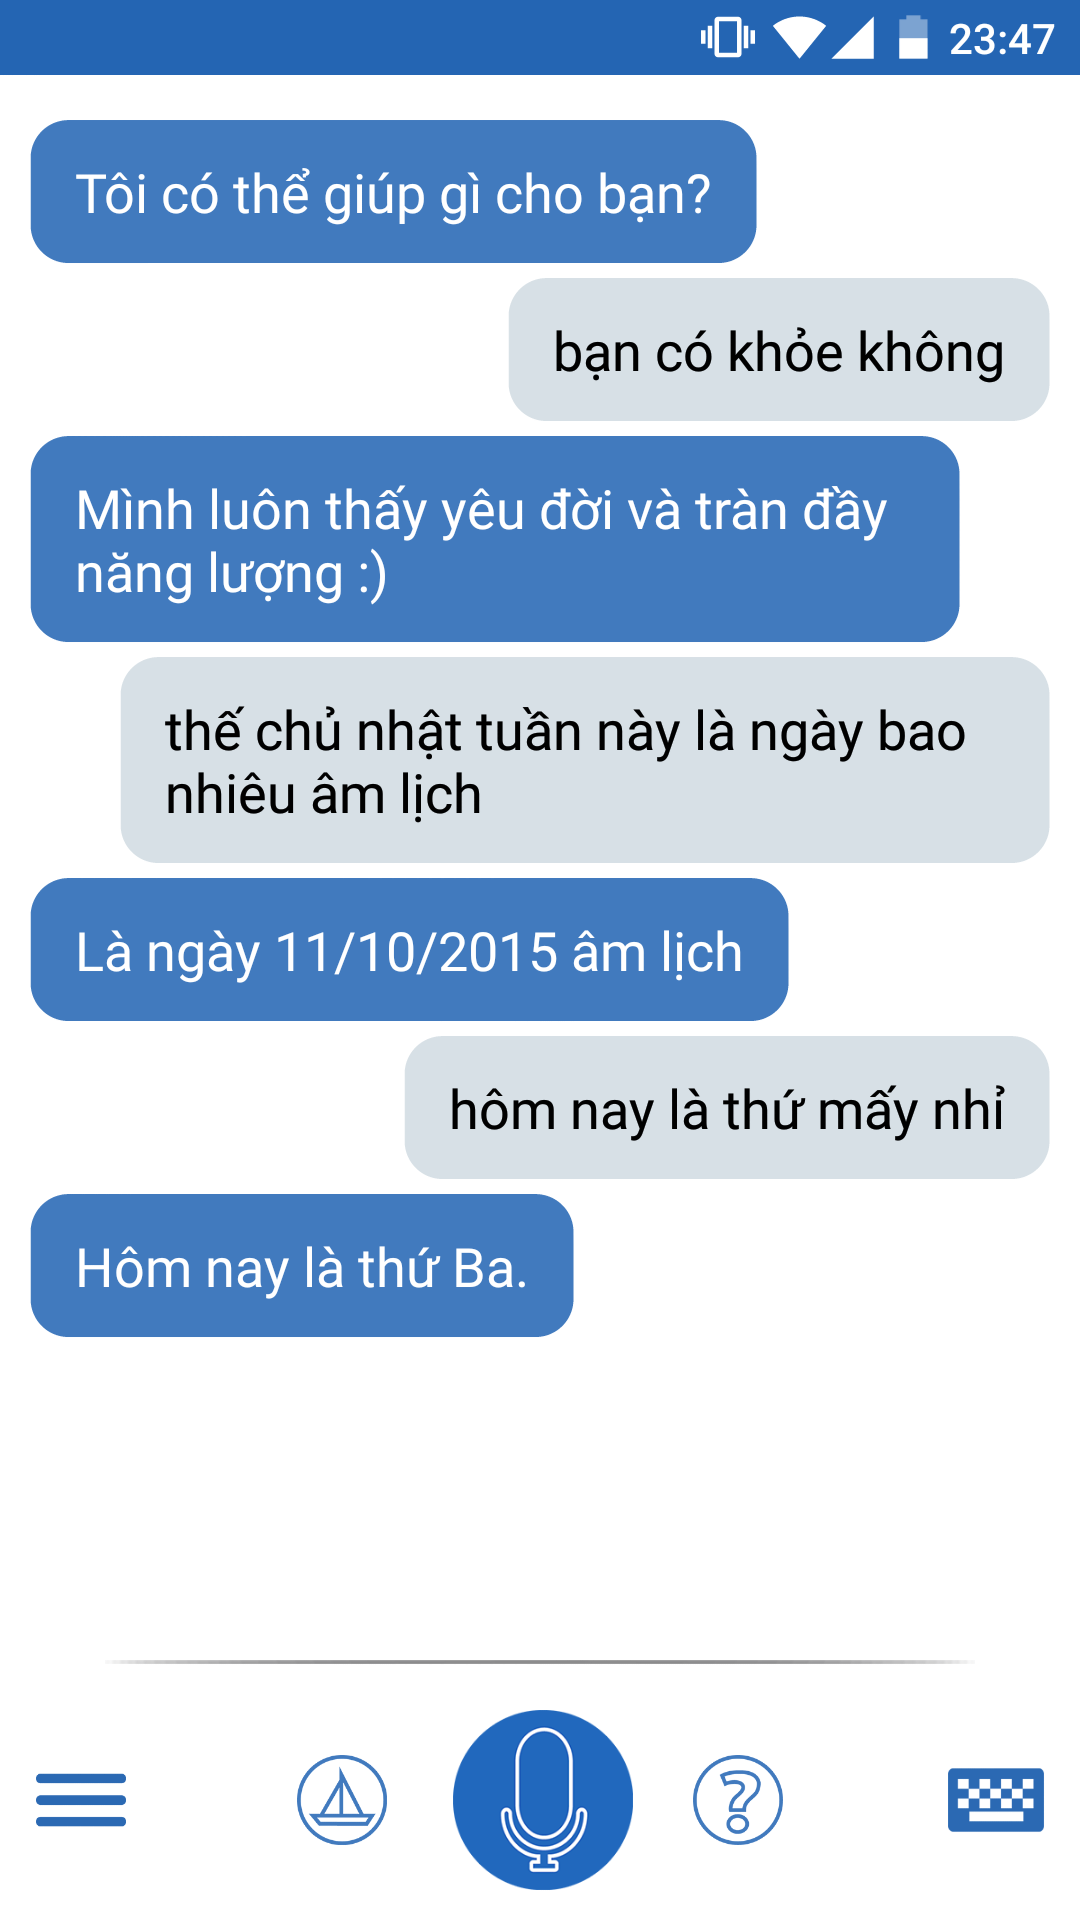
\includegraphics[width=6cm]{Pics/Chap5/vav.png}
	\caption{Màn hình chính của VAV.}
\end{figure}

\subsection{Ứng dụng VietCommand}

VietCommand 

% Chapter 6
\chapter{Kết quả đạt được}

\section{Xây dựng ứng dụng}

Trong phần này, tôi sẽ nói rõ hơn về cấu trúc hệ thống mà đề tài xây dựng để áp dụng những định hướng giải pháp đã nêu ở phần trên. Như mô hình hệ thống đã chỉ ra ở hình \ref{fig:VVC}, hệ thống cần xây dựng một Server trung gian để xử lý các trường hợp nhận diện được từ phía Wit.ai, bên cạnh đó là một ứng dụng Android để thực hiện việc điều khiển tương ứng với các yêu cầu của người dùng. Tuy nhiên, như đã nêu trong \ref{sec:requirement}, để có thể tái sử dụng việc nhận diện yêu cầu bằng giọng nói từ phía người dùng, hệ thống cần tách riêng thành một \texttt{thư viện} (library) Android chuyên để tạo ra dịch vụ nhận diện và phân tích yêu cầu bằng giọng nói, từ đó các ứng dụng như điều khiển điện thoại hay điều khiển nhà thông minh có thể tích hợp một cách dễ dàng.

\subsection{Server trung gian}

Server trung gian được xây dựng bằng ngôn ngữ Javascript với nền tảng \textit{NodeJS} để tạo ra kết nối đến server của Wit.ai, từ đó gửi đi những câu lệnh cần phân tích và nhận lại những dữ liệu đã được Wit.ai phân tích để xử lý, trả lại kết quả cho ứng dụng Android.

\subsubsection{Vài nét về NodeJS}

\textbf{NodeJS} là một nền tảng phía Server được xây dựng dựa trên Javascript Engine (V8 Engine) được phát triển bởi Ryan Dahl năm 2009. Định nghĩa NodeJS bởi tài liệu chính thức như sau:

\begin{formal}
Node.js là một nền tảng dựa vào Chrome Javascript runtime để xây dựng các ứng dụng nhanh, có độ lớn. Node.js sử dụng các phần phát sinh các sự kiện (event-driven), mô hình non-blocking I/O để tạo ra các ứng dụng nhẹ và hiệu quả cho các ứng dụng về dữ liệu thời gian thực chạy trên các thiết bị phân tán.
\end{formal}

Một vài đặc điểm nổi bật của NodeJS:

\begin{itemize}
	\item \textbf{Không đồng bộ và phát sinh sự kiện}: mọi chức năng, hàm trong NodeJS đều không đồng bộ, mọi thứ được chạy liên tiếp nhau trong một luồng duy nhất.
\end{itemize}

\subsubsection{Cấu trúc server trung gian}

Server trung gian được xây dựng theo mô hình MVC cơ bản bao gồm một ChatController để xử lý tương tác với Wit.ai, một UserModel để lưu lại những câu nói của người dùng và một ChatView sử dụng cho việc hiển thị giao diện web của ứng dụng test API trên browser. Bên cạnh đó là một ChatRoute nhằm thực hiện nhiệm vụ điều hướng những request URL được gửi đến bằng phương thức \textit{POST}. Sở dĩ hệ thống sử dụng phương thức này là do chỉ có một loại yêu cầu từ phía người dùng có thể gửi đến nên không cần có sự phân biệt bằng các tham số đầu vào (parameters) được đính kém trên URL, hơn nữa, mọi thông tin trong hệ thống là bảo mật nên không thể sử dụng phương thức GET.

\begin{figure}[H]
	\centering
    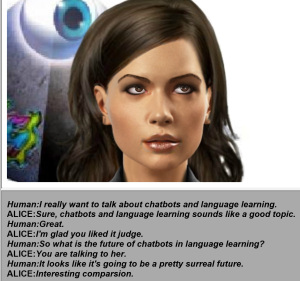
\includegraphics[width=10cm]{Pics/Chap1/alice.jpg}
  	\caption{Giao diện của ứng dụng kiểm thử API.}
\end{figure}

Cụ thể mô hình của hệ thống Server trung gian:

\begin{figure}[H]
	\centering
    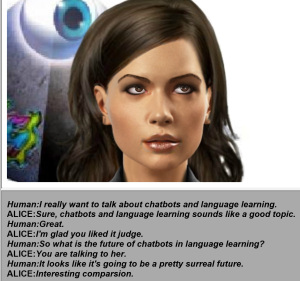
\includegraphics[width=10cm]{Pics/Chap1/alice.jpg}
  	\caption{Giao diện của ứng dụng kiểm thử API.}
\end{figure}

Server trung gian sử dụng 2 node-module chính hỗ trợ việc xây dựng là \textit{Express} và \textit{Node-Wit}, trong đó:

\begin{itemize}
	\item \textbf{Express} hỗ trợ việc tạo ra một server có khả năng nhận yêu cầu từ người dùng, được tạo ra với mô hình MVC cơ bản (đây là việc mà NodeJS không hề hỗ trợ), cung cấp khả năng cài đặt routing (điều hướng) yêu cầu từ người dùng
	\item \textbf{Node-Wit} là một module cung cấp bởi Wit.ai, tạo ra một class Wit chứa các phương thức giao tiếp với Wit.ai server, để có thể gửi và nhận những kết quả phân tích từ Wit.ai
\end{itemize}

\subsubsection{Cấu trúc dữ liệu}

\begin{lstlisting}[frame=lines, basicstyle=\footnotesize\ttfamily, numbers=left, numberstyle=\tiny\color{black},caption= {Cấu trúc một API trả về}, backgroundcolor=\color{background}]
{
  "context": {
    <intent_context>
  },
  "response": {
    "text": <content>
  },
  "status": <status_number>,
  "entities": {
    <entity_1>: [
      {
        "confidence": 0.9941168619530284,
        "type": "value",
        "value": <entity_1_value>,
        "suggested": true
      }
    ],
    <entity_2>: [
      {
        "confidence": 0.9973928924388795,
        "value": <entity_2_value>
      }
    ]
  }
}
\end{lstlisting}

\subsection{Xây dựng thư viện}

\subsection{Tích hợp thư viện}

\section{Cài đặt thuật toán chọn lọc kết quả}

\subsection{Công cụ SRILM}
SRILM là bộ công cụ để xây dựng và áp dụng các mô hình ngôn ngữ thống kê. Bộ công cụ này được phát triển bởi “Phòng thí nghiệm và nghiên cứu công nghệ giọng nói SRI” từ năm 1995, có thể cài đặt và chạy trên nền tảng Linux cũng như Windows.
Hệ thống sẽ sử dụng SRILM làm công cụ huấn luyện mô hình ngôn ngữ dựa trên tập dữ liệu đã được nạp cho chatbot trên Wit.ai (nền tảng phân tích yêu cầu từ phía người dùng - sẽ được nêu rõ trong phần sau). SRILM bao gồm các thành phần:

\begin{itemize}
	\item Một tập hợp các thư viện C++ giúp cài đặt mô hình ngôn ngữ, hỗ trợ cấu trúc dữ liệu và các tiện ích nhỏ
	\item Một tập hợp các chương trình thực hiện nhiệm vụ xây dựng mô hình ngôn ngữ, huấn luyện và thử nghiệm mô hình ngôn ngữ trên dữ liệu …
\end{itemize}

Ở đây, chúng tôi sử dụng duy nhất một chức năng của SRILM là huấn luyện và xây dựng một mô hình ngôn ngữ (sẽ lưu lại dưới dạng tệp .lm) để phục vụ cho việc tính xác suất về sau. Đó là chức năng \texttt{ngram-count}. Câu lệnh \texttt{ngram-count} nhận thông tin đầu vào là một file dạng text chứa các câu muốn huấn luyện và thống kê tần số xuất hiện của các cụm N-gram. Kết quả của việc thống kê được ghi lại vào tệp .count hoặc được sử dụng với các lựa chọn về phương pháp “làm mịn” để xây dựng nên một mô hình ngôn ngữ được ghi lại vào tệp .lm. Mô hình ngôn ngữ này sau đó sẽ được sử dụng để tính xác suất cho các câu trong tập kiểm thử và chọn lựa ra câu có xác suất lớn nhất.

Tệp mô hình ngôn ngữ đã được huấn luyện có dạng như sau:
\begin{lstlisting}[frame=lines, basicstyle=\footnotesize\ttfamily, numbers=left, numberstyle=\tiny\color{black},caption= {Cấu trúc một mô hình ngôn ngữ}, backgroundcolor=\color{background}]
	\data\
	ngram 1 = n1
	ngram 2 = n2
	...
	ngram n = nN

	\1-grams:
	logp w  [bow]
	...

	\2-grams:
	logp w1w2 [bow]
	...

	\N-grams:
	logp w1w2 ... wN [bow]
	...

	\end
\end{lstlisting}
		
Trong đó, phần data chính là số lượng các cụm n-gram đã thống kê được, tiếp theo là chi tiết từng cụm n-gram có độ dài từ 1 đến n. Mỗi dòng trong chi tiết từng cụm n-grams bắt đầu bằng một số logarit cơ số 10 xác suất của cụm N-grams, tiếp theo là n từ w1 đến wn của cụm N-grams đó, và cuối cùng là trọng số truy hồi của cụm N-grams (có thể có).

Hệ thống sử dụng SRILM để huấn luyện và xây dựng mô hình ngôn ngữ và đưa mô hình ngôn ngữ đó vào trong ứng dụng trên điện thoại thông minh Android. Với mỗi tập kết quả trả về từ phía Google, ta tính logarit cơ số 10 xác suất của các câu trong tập kết quả bằng công thức (2) và lựa chọn câu có logarit lớn nhất. Câu được lựa chọn ra sẽ được dùng để mang đi phân tích yêu cầu từ phía người dùng.

\subsection{Tính xác suất}



\section{Xây dựng kiến thức cho chatbot}

\subsection{Vài nét về Wit.ai}

\begin{figure}[H] \label{fig:mainboard-wit}
	\centering
	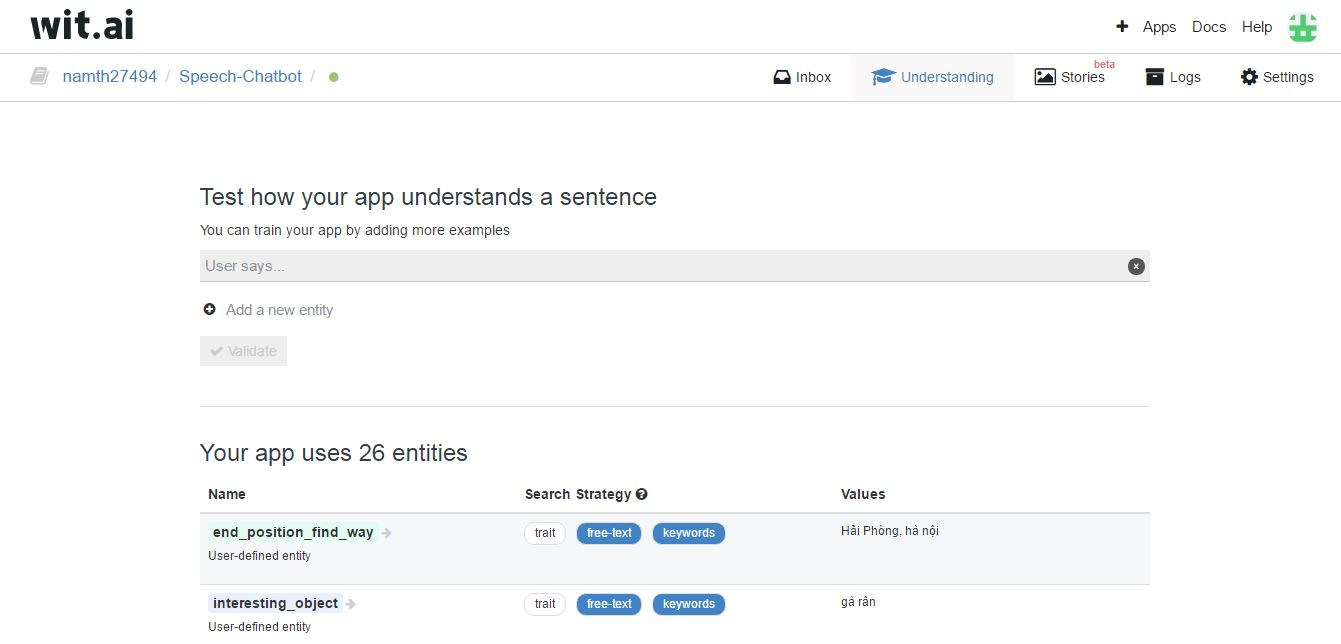
\includegraphics[width=10cm]{Pics/Chap6/wit-mainboard.JPG}
	\caption{Màn hình chính của Wit.ai.}
\end{figure}

\subsection{Sử dụng Wit.ai}

Đối tượng chính của Wit.ai là các entity. Entity là đơn vị khi Wit.ai phân tích một câu trong tập dữ liệu huấn luyện. Có 3 kiểu entity:

\begin{itemize}
	\item \textbf{trait}: là các entity dự đoán và phân loại các câu có tính chất và trường hợp tương tự nhau, tuy cách diễn đạt khác nhau nhưng đều được nhận ra là cùng một ý nghĩa
	\item \textbf{free-text}: là entity để trích ra một xâu kí tự con (substring) trong cả câu, và xâu con này chưa từng được định nghĩa trước trong một danh sách nào cả
	\item \textbf{keywords}: khi giá trị của entity đã được định nghĩa trong một danh sách có trước và chúng ta chỉ cần tìm một xâu con trùng khớp với entity này trong câu
\end{itemize}

\begin{figure}[H] 
	\centering
	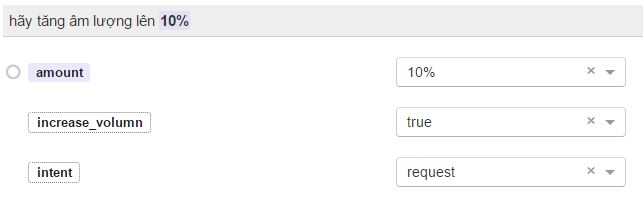
\includegraphics[width=10cm]{Pics/Chap6/wit.JPG}
	\caption{Các Entity khi phân tích một câu trong Wit.ai.}
	\label{fig:entity}
\end{figure}

Hình \ref{fig:entity} là một ví dụ trong việc phân tích một câu yêu cầu trong Wit.ai. Ta thấy \textit{intent} và \textit{increase\_volumn} là 2 entity thuộc kiểu trait, với các câu tương tự như ``hãy tăng âm lượng'' hoặc ``cho âm thanh lớn lên 20\%'' thì Wit.ai đều phân loại các câu đó vào 2 kiểu entity này: đây là một yêu cầu và yêu cầu đó là muốn tăng âm lượng. Entity \textit{amount} thuộc kiểu free-text kết hợp với keyword để nhận diện được từ ngữ làm đầu vào cho các hành động khi thực hiện yêu cầu, như ví dụ là tăng âm lượng lên 10\%. Thông qua việc phân tích này, yêu cầu từ phía người dùng sẽ được nhận dạng mặc dù người dùng có những cách diễn đạt khác nhau, từ đó hệ thống điều khiển có thể tùy vào những trường hợp được nhận dạng sẽ đưa ra các hành động tương ứng và phù hợp.

Một đặc điểm nổi bật của AIML chính là việc chọn ra câu trả lời phù hợp với câu nói của người dùng. Việc này được Wit.ai chuyển thành các Story, nơi mà quy định cách trả lời của bot trong các trường hợp cụ thể. 
 
\begin{figure}[H] \label{fig:story-wit}
	\centering
	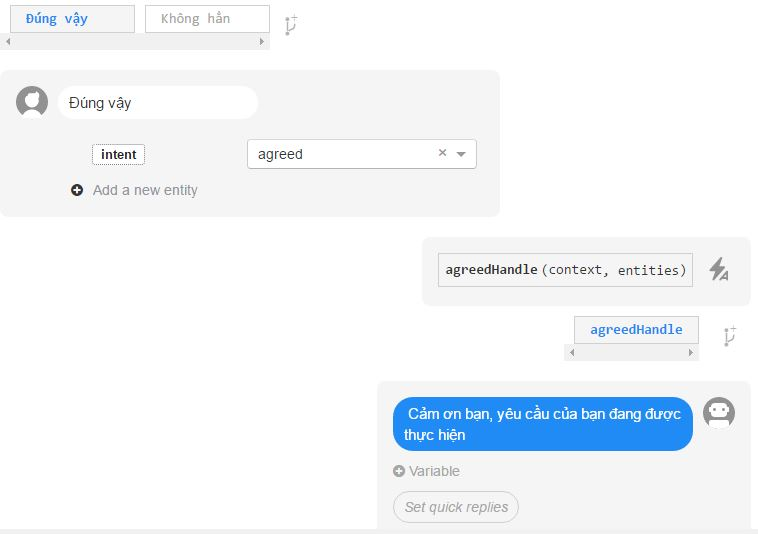
\includegraphics[width=10cm]{Pics/Chap6/story.JPG}
	\caption{Cài đặt story trong Wit.ai.}
\end{figure}

Với các story, chatbot sẽ biết được nên trả lời như thế nào trong từng trường hợp cụ thể. Chúng ta có thể tạo ra nhiều story để quy định cách trả lời của chatbot, ví dụ như story \textit{Greeting} sẽ tập trung xử lý các câu liên quan đến chào hỏi như ``Xin chào'' hay ``Tên bạn là gì?'' \ldots, trong khi đó story \textit{RequestHandle} sẽ quy định cách trả lời của chatbot trong những trường hợp người dùng đưa ra yêu cầu. Mọi kiến thức của chatbot đều được cập nhật thông qua giao diện chính của Wit.ai. \\[0.3mm]

\noindent \textbf{Vậy làm thế nào để cập nhật những câu nói mà hệ thống chưa phân tích được?\\[0.3cm]}

Với những câu chưa từng xuất hiện hoặc còn nhập nhằng trong việc phân tích, Wit.ai sẽ đẩy về phần Inbox, và tại đây chúng ta sẽ thực hiện phân tích và phân loại những câu này để Wit.ai tiếp tục học và phát triển.

\begin{figure}[H] \label{fig:inbox-wit}
	\centering
	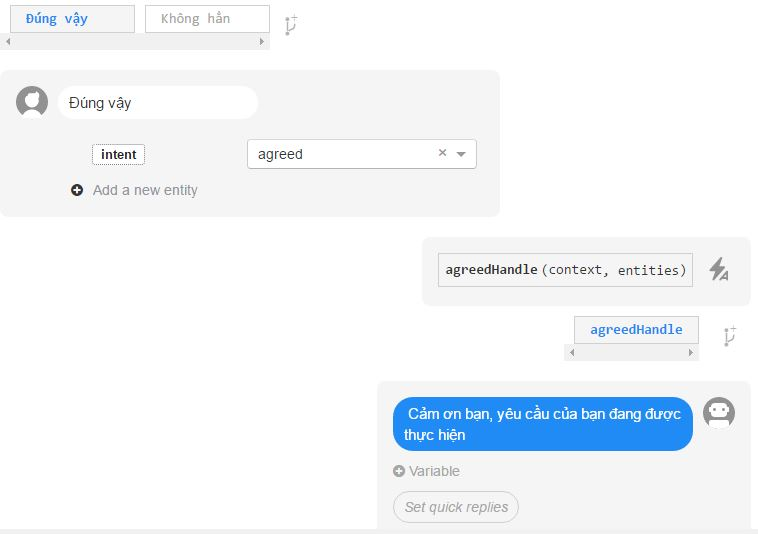
\includegraphics[width=10cm]{Pics/Chap6/story.JPG}
	\caption{Cập nhật kiến thức cho chatbot trong Inbox.}
\end{figure}

% Chapter 7
\chapter{Cài đặt và đánh giá} \label{chap:setup}

\section{Đánh giá độ chính xác của mô hình ngôn ngữ}

Trong phần thực nghiệm, chúng tôi lấy mẫu từ hơn 1000 câu bao gồm các trường hợp đã huấn luyện cho chatbot để làm đầu vào cho việc huấn luyện mô hình ngôn ngữ. Cụ thể số lượng các cụm n-gram như sau:
\begin{table}[h]
	\caption{Số lượng các cụm n-gram trong tập huấn luyện}
	\centering
	\begin{tabular}{ | C | C | }
	\hline
	N & Số lượng \\
	\hline
	1 & 573 \\
	\hline
	2 & 1272 \\
	\hline
	3 & 492 \\
	\hline
	\end{tabular}
\end{table}

Sử dụng mẫu này để huấn luyện các mô hình ngôn ngữ theo các phương pháp ``làm mịn'' khác nhau. Sau đó, một tập văn bản kiểm thử được đưa vào bao gồm 200 tập câu khác nhau, mỗi tập câu là một tập kết quả từ phía Google Speech Recognition trả về để tính xác suất dựa trên các mô hình ngôn ngữ đã huấn luyện và chọn ra các câu hợp lí nhất dựa vào hàm tính Perplexity:
\begin{align*}
PP(W) &= P(w_1w_2 \ldots w_N)^{\frac{-1}{N}} \\
	&= \sqrt[N]{\frac{1}{P(w_1w_2 \ldots w_N)}}
\end{align*}

Perplexity là nghịch đảo của xác suất của tập văn bản kiểm thử, và được chuẩn hóa bằng số lượng các từ có trong văn bản.
==> Perplexity càng nhỏ thì xác suất xảy ra càng lớn. Như đã nêu ở trên, thay việc nhân các xác suất bằng việc cộng các logarit cơ số 10 của xác suất giúp cho việc tính toán nhanh hơn. Vì vậy công thức tính perplexity chuyển thành:
\[PP(W) = 10^{(\frac{-\log\textit{prob}}{\textit{words} - \textit{OOVs}})}\]

Trong đó \textit{words} là số các từ trong câu, \textit{OOVs} là số các từ chưa từng xuất hiện trong tập học. Những từ này gây ra xác suất bằng 0, vì vậy logarit cơ số 10 sẽ là âm vô cùng, nên khi tính toán sẽ bỏ qua. Từ đó ta có bảng thống kê kết quả nhận biết của các phương pháp với 200 bộ dữ liệu kiểm thử:
\begin{table}[h]
	\caption{Kết quả đánh giá tập kiểm thử của các phương pháp làm mịn}
	\centering
	\begin{tabular}{ | c | c | }
	\hline
	Phương pháp làm mịn & Độ chính xác \\
	\hline
	Good-Turing Discount & 74\% \\
	\hline
	Witten-Bell & 80\% \\
	\hline
	Kneser-Ney & 70\% \\
	\hline
	\end{tabular}
\end{table}

Qua đó ta thấy được việc ưu tiên và chuyển xác suất quá nhiều cho các cụm N-gram chưa từng xuất hiện làm giảm khả năng loại bỏ đi những cụm từ không cần thiết và không xuất hiện trong tập huấn luyện. Tuy nhiên việc áp dụng mô hình ngôn ngữ cũng đã đánh giá được phần nào những câu nói phù hợp trong tập dữ liệu trả về nhưng lại không được đánh giá cao do có sự nhập nhằng trong ngữ điệu và âm lượng của người dùng. 

\section{Đánh giá hệ thống}

Hệ thống được chạy trên thiết bị Android 6.0 với tốc độ trả lời yêu cầu người dùng trung bình là 1268ms, là tốc độ có thể chấp nhận được với một hệ thống điều khiển bằng giọng nói.

\stopcontents[parts]

\chapter*{Kết luận}
\addtocontents{toc}{\bigskip}
\addcontentsline{toc}{chapter}{Kết luận}

Qua quá trình nghiên cứu và xây dựng ứng dụng ``Chatbot điều khiển điện thoại bằng Tiếng Việt'', em đã rút ra được những bài học vô cùng quý giá, đặc biệt trong lĩnh vực xử lý ngôn ngữ tự nhiên nói riêng và lĩnh vực trí tuệ nhân tạo nói chung. Thông qua việc tìm hiểu những kỹ thuật xử lý cơ bản trong xử lý ngôn ngữ tự nhiên, em đã nắm bắt được một phần những kiến thức nền tảng trong việc xây dựng các ứng dụng có trí thông minh, khả năng thay thế con người để hoàn thành những nhiệm vụ cụ thể.

Ứng dụng ``Chatbot điều khiển điện thoại bằng Tiếng Việt'' mới chỉ được xây dựng một cách sơ khai với mô hình hệ thống còn nhiều thiếu sót, tuy nhiên kết quả thực tiễn đem lại vẫn rất khả quan, mở ra những hướng đi trong việc sử dụng giọng nói Tiếng Việt để điều khiển những vật dụng thông minh ngay tại Việt Nam.

Trong quá trình nghiên cứu và phát triển ứng dụng không tránh khỏi những sai sót, em rất mong nhận được sự góp ý từ thầy cô và các bạn để có thể hoàn thiện được ứng dụng hơn nữa về mọi mặt, cả trong khả năng thông minh cũng như tối ưu hóa tốc độ của ứng dụng. \\[0.4cm]
\noindent \textbf{\large Định hướng phát triển\\[0.4cm]}
Ứng dụng ``Chatbot điều khiển điện thoại bằng Tiếng Việt'' còn cần thêm rất nhiều dữ liệu trả lời và phân tích yêu cầu từ phía người dùng, hơn nữa, mô hình hệ thống của ứng dụng chưa thực sự tốt, vì vậy em xin đề xuất một số định hướng phát triển trong tương lai để ứng dụng trở nên hoàn thiện hơn:

\begin{itemize}
	\item Xây dựng khả năng tự học cho chatbot.
	\item Chuyển toàn bộ nhiệm vụ xử lý giọng nói cũng như phân tích yêu cầu về cho server để thuận tiện cho việc cập nhật mô hình ngôn ngữ và phát triển thư viện tích hợp.
\end{itemize}

\begin{thebibliography}{9}
\bibitem{robustasr} 
Andrew L. Maas , Quoc V. Le, Tyler M. O’Neil , Oriol Vinyals, Patrick Nguyen and Andrew Y. Ng. 
\textit{Recurrent Neural Networks for Noise Reduction in Robust ASR}. 
Google Research, 2012.

\bibitem{bayesLMformobile} 
Cyril Allauzen and Michael Riley. 
\textit{Bayesian Language Model Interpolation for Mobile Speech Input}. 
Google Research, 2011.

\bibitem{justspeak} 
Yu Zhong, T.V. Raman, Casey Burkhardt, Fadi Biadsy and Jeffrey P. Bigham. 
\textit{JustSpeak: Enabling Universal Voice Control on Android}. 
Google Research, 2014.

\bibitem{neuralLM} 
Yoshua Bengio, Réjean Ducharme, Pascal Vincent and Christian Jauvin. 
\textit{A Neural Probabilistic Language Model}. 
Journal of Machine Learning Research, 2003.

\bibitem{vietnameseLM} 
Cao Van Viet, Do Ngoc Quynh and Le Anh Cuong. 
\textit{Building and Evaluating Vietnamese Language Models}. 
VNU Journal of Science: Mathematics - Physics, [S.l.], ISSN 2588-1124, 2011.

\bibitem{chappie} 
Bibek Behera. 
\textit{Chappie - A Semi-automatic Intelligent Chatbot}. 
2016.

\bibitem{charliechatbot} 
Fernando A. Mikic, Juan C. Burguillo, Martín Llamas, Daniel A. Rodríguez and Eduardo Rodríguez. 
\textit{CHARLIE: An AIML-based Chatterbot which works as an Interface among INES and Humans}. 
EAEEIE Annual Conference, 2009.

\end{thebibliography}

\addcontentsline{toc}{chapter}{Tài liệu tham khảo}

\end{document}